\documentclass[a4paper,twoside]{report}
\usepackage[print]{autiwa}

\setcounter{secnumdepth}{2}
\usepackage{minitoc}
\setcounter{minitocdepth}{1}

\fancyhead[LE]{}

\makeatletter

% macros qui servent à la mise en page, elles ne doivent pas être utilisées directement
\newcommand{\preparationTopSep}{\vspace{.2cm} \hrule height0.25pt width\hsize \vspace{1em}}
\newcommand{\statistiqueTopSep}{\vspace{.3cm} \hrule height1pt width\hsize \nobreak \vskip\parskip \vspace{.3cm}}
\newcommand{\ingredientsTopSep}{\vspace{.4cm} \hrule height0.75pt width\hsize\vspace*{1\p@}\hrule height0.25pt width\hsize \vspace{1em}}
\newcommand{\partStyle}{\bfseries \large}

% redéfinition d'une nouvelle commande de section qui n'a pas de numérotation, est centrée, avec mise en page modifiée. C'est pour afficher le titre des recettes et qu'elles apparaissent dans le menu. J'avais fait avec addcontentline mais la référence n'était pas bonne et pointait sur la page précédente parfois. Bref, pas propre.
\newcommand\nomRecette{\@startsection {section}{6}{\z@}{0ex}{2.3ex }%
	{\reset@font\Huge\bfseries\centering}}

\usepackage{bbding}%to add \FiveStar and \FiveStarOpen
\newcommand{\note}[1]
{
  \ifthenelse{\equal{#1}{0}}{non testé}{}
  \ifthenelse{\equal{#1}{1}}{\FiveStar\FiveStarOpen\FiveStarOpen\FiveStarOpen\FiveStarOpen}{}
  \ifthenelse{\equal{#1}{2}}{\FiveStar\FiveStar\FiveStarOpen\FiveStarOpen\FiveStarOpen}{}
  \ifthenelse{\equal{#1}{3}}{\FiveStar\FiveStar\FiveStar\FiveStarOpen\FiveStarOpen}{}
  \ifthenelse{\equal{#1}{4}}{\FiveStar\FiveStar\FiveStar\FiveStar\FiveStarOpen}{}
  \ifthenelse{\equal{#1}{5}}{\FiveStar\FiveStar\FiveStar\FiveStar\FiveStar}{}
}

\newcommand{\ingredient}[1][]{\ifthenelse{\equal{#1}{}}{\item }{\vspace{1ex}\hrule\vspace{1ex}\item[\textcurrency]\textbf{#1}}}

\newcommand{\etape}[1][]{\ifthenelse{\equal{#1}{}}{\item }{\item[\textbf{#1}]}}

% Environnement qui crée une nouvelle recette. Ingrédients, étape, cuisson etc doivent être contenus dans un environnement recette.
\newenvironment{recette}[4]{\newpage \nomRecette{#1}\statistiqueTopSep\note{#2}\ifthenelse{\equal{#4}{}}%
{\hfill
\includegraphics[width=1em]{figures/logo_minuterie.pdf} \; \begin{itshape}\textbf{Préparation \& Cuisson :} #3\end{itshape}}%if none
{\hfill
\includegraphics[width=1em]{figures/logo_minuterie.pdf} \; \begin{itshape}\textbf{Préparation :} #3 \hfill 
\includegraphics[width=1em]{figures/logo_minuterie.pdf} \;\textbf{Cuisson :} #4\end{itshape}}}{}

% Environnement pour la mise en page des ingrédients. Un argument optionnel de l'environnement permet de spécifier pour combien de personnes sont les doses. Les entrées de cet environnement doivent être ``\ingredient nom de l'ingrédient''. Si on veut séparer les ingrédients, pour dénoter deux sortes de choses, ingrédient pour une sauce et une pâte par exemple, il faut faire une ligne du style \ingredient[pour la sauce] afin de séparer.
\newenvironment{ingredients}[1][]{\ingredientsTopSep{\partStyle Ingrédients\ifthenelse{\equal{#1}{}}{}{ (#1)}}\begin{multicols}{2}\begin{itemize}\renewcommand{\labelitemi}{$\bullet$}}{\end{itemize}\end{multicols}}

% Environnement pour mettre en page la préparation du plat. Les entrées sont de la forme ``\etape texte de l'étape``. Si on veut séparer les étapes, pour dénoter un groupement d'étape par exemple, il faut faire une ligne du style \etape[pour la sauce] afin de séparer.
\newenvironment{preparation}{\preparationTopSep{\partStyle Préparation }\vspace{0.5em}\begin{enumerate}}{\end{enumerate}}

% À utiliser si on souhaite faire une mise en page un peu plus évoluée, avec deux listes par exemples.
\newenvironment{preparation*}{\preparationTopSep{\partStyle Préparation }\vspace{0.5em}\par}{}

% Environnement pour mettre en page la cuisson du plat
\newenvironment{cuisson}{\bigskip{\bfseries \large Cuisson }\par}{}
\makeatother

%TODO Faire une commande pour que dans l'index on voit la liste des recettes en fonction de la note qu'elles ont. 

\title{Recettes de Cuisine}
\author{Autiwa}
\begin{document}
\begin{titlepage}
\begin{center}
~
\vfill
% Upper part of the page
\begin{figure}[t]
\centering

\includegraphics[width=0.15\textwidth]{logo-autiwa.pdf}%chemin absolu de l'image pour que l'on puisse appeler ce fichier depuis plusieurs dossiers différents.
\end{figure}

% Title
\HRule \\[0.4cm]
{ \huge \bfseries \makeatletter\@title\makeatother}\\[0.4cm]

\HRule \\[0.75cm]
{\large \today}\\[0.75cm]
\makeatletter
\@author
\makeatother
\vfill
\vfill
~
% Bottom of the page


\end{center}
\end{titlepage}

\dominitoc
\tableofcontents
\chapter{Plat Principal}
\minitoc

\begin{recette}{Blanquette de Veau}{2}{20 min}{2h}
\begin{ingredients}
\ingredient 1,2 kg d'épaule ou de tendron de veau coupé en morceaux
\ingredient 1 carotte
\ingredient 2 blancs de poireaux
\ingredient 1 gros oignon
\ingredient 1 gousse d'ail
\ingredient 2 échalotes
\ingredient 1 brin de céleri
\ingredient 1 bouquet garni
\ingredient 1 bouquet de persil
\ingredient 1 citron
\ingredient 300 g de champignons de Paris
\ingredient 3 cuillères à soupe de vin blanc sec
\ingredient 2 jaunes d'oeufs
\ingredient 1 dl de crème fraîche
\ingredient 1 cuillère à soupe de farine
\ingredient 70 g de beurre
\end{ingredients}

\begin{preparation}
\etape Pelez carotte, ail, échalotes et oignon. Hachez ce dernier ainsi que les blancs de poireaux. Coupez les échalotes et la carotte en deux.

\etape Portez à ébullition 2 litres d'eau dans un grand faitout, plongez-y les morceaux de viande pendant environ une minute pour les blanchir (blanchir la viande permet d'éliminer les éventuelles impuretés tout en la rendant plus ferme). Egouttez la viande, rincez-la sous l'eau froide et jetez l'eau de cuisson.

\etape Replacez la viande dans le faitout rincé. Ajoutez oignon et poireaux hachés, carottes, échalotes, ail, céleri et bouquet garni. Salez, poivrez et mouillez avec le vin. Ajoutez de l'eau pour que la viande et les légumes soient immergés.

\etape Couvrez. Portez à ébullition et laissez cuire 1 h 30. Faites cuire dans une poêle, avec 30 g de beurre, les champignons coupés et citronnés 10 min.

\etape Préparez un roux blond : faites fondre le reste de beurre dans une casserole, saupoudrez-le avec la farine, mélangez vivement au fouet, puis laissez refroidir. Quand la viande est cuite, mettez-la dans une passoire avec les légumes et récupérez le bouillon de cuisson. Délayez le roux avec ce bouillon et amenez à ébullition en fouettant.

\etape Remettez la viande et tous les légumes dans le faitout après avoir retiré bouquet garni, ail, céleri et carotte. Ajoutez les champignons, versez la sauce et réchauffez le tout 10 à 15 mn.

\etape Juste avant de servir mélangez la crème et les jaunes d'oeufs, incorporez-les à la sauce en tournant sans laisser bouillir. Ajoutez quelques gouttes de jus de citron. Servez dans un plat creux avec du persil.
\end{preparation}



\end{recette}

\begin{recette}{Brandade de morue}{0}{24h}{30 min}
\begin{ingredients}
\ingredient $400$ g de morue salée
\ingredient 2 gousses d'ail
\ingredient persil
\ingredient $10$ cl de crème fraiche
\ingredient $\sfrac{1}{2}$ verre ($12.5$ cl) d'huile d'olive
\ingredient 1 citron
\ingredient $600$ g de pomme terre
\ingredient laurier
\ingredient beurre
\end{ingredients}

\begin{remarque}
On peut remplacer la morue par de la lotte (qui est environ 2 fois moins chère que la morue). Par contre, c'est beaucoup moins salé du coup\dots
\end{remarque}


\begin{preparation}
\etape Mettre la morue à déssaler 24 heures à l'avance. Changer l'eau 3 ou 4 fois.
\etape Le lendemain, préparer l'ail et le persil
\end{preparation}

\begin{cuisson}
\begin{enumerate}
\item Faire cuire la morue dans une casserole d'eau froide au départ, avec deux feuilles de laurier. Porter à ébullition et laisser cuire à petite ébulition pendant 10 minutes.
\item En parallèle, faire cuire les pommes de terre dans une casserole d'eau pendant 20 minutes.
\item Egoutter puis émietter la morue dans une casserole contenant l'ail et le persil. mettre un peu de jus de citron.
\item Ajouter progressivement l'huile d'olive en tournant rapidement avec une cuillère. Cuire à petit feu pendant quelques minutes tout en écrasant les morceaux contre la paroi de la casserole.
\item Ecraser les pommes de terre à la fourchette et mettre la purée ainsi formée dans la casserole.
\item Ajouter la crème fraîche et tourner à nouveau pour bien mélanger les ingrédients. Si le mélange est trop sec et ne forme pas une purée, ajouter un peu d'eau de cuisson des pommes de terre.
\item Placer dans un plat à gratin, ajouter quelques fines lamelles de beurre dessus et faire gratiner pendant 4 minutes
\end{enumerate}
\end{cuisson}

\end{recette}

\begin{recette}{Calamars à l'armoricaine}{3}{}{}
\begin{ingredients}
\ingredient 1 boite moyenne de tomates en dés
\ingredient 1 boite de coulis de tomate (ou une 2\ieme boite de tomates en dés)
\ingredient 500g de calamars
\ingredient 4 échalotes
\ingredient 3 ou 4 oignons
\ingredient 1 gousse d'ail
\ingredient 20cl de vin blanc
\ingredient 5 cl de cognac
\ingredient 20g de beurre
\ingredient sel, poivre, huile d'olive, piment ou sauce piquante, sucre
\end{ingredients}

\begin{remarque}
J'ai mis 750g de calamars (une poche et demie) pour 4. Ça diminue beaucoup durant la cuisson. Donc en gros, on peut mettre une poche, suivant le poids de la poche, c'est pas très grave qu'il y en ait un peu moins ou un peu plus.
\end{remarque}


\begin{preparation}
\etape Pelez et hachez lail, l'oignon et l'échalote (avec un robot, pas besoin de s'embêter).
\etape Faites revenir les ronds de calamars (sans les décongeler s'ils le sont) dans le beurre et l'huile pendant 2 minutes environ. (dans la pratique, s'ils sont surgelés, faut au moins qu'ils soient décongelés). Une fois fait, réservez les calamars et le jus rendu dans un récipient.
\etape Faites revenir à feu doux la mixture oignon+échalote+ail. Rajoutez un peu d'eau si besoin pour pas que ça accroche.
\etape Une fois légèrement transparent, à peine doré, rajoutez les calamars, laissez un peu réchauffer, puis rajouter le cognac et faites flamber.
\etape Ajoutez les tomates en dés, le vin blanc, salez, poivrez et laissez mijoter à couvert pendant une heure environ.
\etape Enfin, durant la cuisson, une fois que tout est un peu mélangé, goutez. Compensez les gouts avec sel poivre et piment fort. Et s'il y a une sorte d'aigreur, rajoutez un peu de sucre afin de l'éliminer. Bien entendu, goutez jusqu'à ce que ça vous convienne.
\end{preparation}

\end{recette}

\begin{recette}{Canard à la Bourguignonne}{5}{}{}
% (Excellent)

\begin{ingredients}
\ingredient $1$ canard
\ingredient $75$ g de beurre
\ingredient $2$ oignons
\ingredient une cuillère à café de fond de veau
\ingredient $1$ carotte
\ingredient $2$ gousses d'ail
\ingredient $15$ cl de madère
\ingredient $10$ cl de cognac
\ingredient $50$ g d'olives dénoyautées
\ingredient sel, poivre du moulin
\end{ingredients}

\begin{preparation}
\etape Découpez le canard en morceaux et faites-le revenir dans du beurre avec des oignons hachés. Le feu doit être relativement fort. Pas besoin que la viande soit cuite à l'intérieur, c'est juste pour faire dorer.
\etape Lorsque les morceaux sont bien dorés, ajoutez de l'extrait de viande, une carotte, deux gousses d'ail et un verre de madère.
\etape En fin de cuisson (au bout d'environ 20 minutes), lorsque la sauce sera bien réduite, ajoutez un petit verre de cognac et 50 g d'olives dénoyautées.
\etape Servez avec des croûtons frits.
\end{preparation}

\begin{remarque}
Mon avis personnel est que cette sauce va très bien avec du riz.
\end{remarque}

\end{recette}

\begin{recette}{Canard aux pruneaux}{3}{}{}
% (recette que j'ai inventé)
\begin{ingredients}
\ingredient morceaux de canards (8 manchons par exemple)
\ingredient 3 échalottes
\ingredient 150g de champignons
\ingredient 25cl de bouillon de volaille
\ingredient une cuillère à café de fond de veau
\ingredient 10cl de cognac
\ingredient 20cl de vin blanc
\ingredient pruneaux
\ingredient huile, beurre, sel, poivre
\end{ingredients}

\begin{preparation}
\etape Faites revenir les morceaux de canard à feu vif dans une sauteuse avec moitié beurre moitié huile d'olive. Une fois bien doré, réservez les.
\etape déglacez avec le cognac, et mettez les échalottes et les champignons dans la sauteuse. Couvrez et laissez mijoter jusqu'à ce que ce soit cuit (en remuant de temps en temps)
\etape rajoutez le bouillon de volaille, le vin blanc, le fond de veau et les pruneaux. Remuez, puis rajoutez les morceaux de canard.
\etape Laissez mijoter 30 minutes environ (ou plus longtemps si les morceaux sont plus gros et plus longs à cuire).
\end{preparation}

\end{recette}

\begin{recette}{Canard laqué}{3}{10 min + 6h}{2h}

\begin{ingredients}
\ingredient 1 cuillerée à café de sel
\ingredient 1 cuillerée à soupe de poudre aux cinq-épices (voir sur le Site : Description de quelques produits exotiques)
\ingredient 1-2 verre de miel liquide (ou mélasse ou sucre roux)
\ingredient 1-3 de verre de sauce de soja 5 cuillerées à soupe de vinaigre blanc
\ingredient 2 cuillerées à soupe de vermouth (ou porto) blanc
\ingredient 2 cuillerées à soupe de fécule
\ingredient 2 gousses d'ail écrasées et finement hachées
\ingredient 10 g de levure vivante (ou levure chimique)
\end{ingredients}

\begin{preparation}
\etape Plongez le canard entier dans de l'eau bouillante 30 secondes puis lavez et essuyez l'intérieur et l'extérieur avec des serviettes en papier.
\etape En utilisant un poinçon, faites de multiples trous dans la peau et les muscles du volatile.
\etape Mélangez intimement dans un bol tous les éléments de la laque.
\etape Mettez le canard dans un plat profond. Arrosez-le avec la laque; versez aussi un peu de laque dans sa cavité.
\etape Laissez mariner le canard au moins 6 heures, au réfrigérateur de préférence, en le retournant et l'arrosant de laque de temps en temps.
\end{preparation}

\begin{cuisson}
\begin{enumerate}
\item Embrochez le canard et faites-le cuire en rôtissoire préchauffée et réglée à 6 (voir Remarque 5).
\item La cuisson dure environ 2 heures, jusqu'à ce que la peau du canard devienne luisante et soit d'un brun assez foncé.
\item Après la première heure de cuisson, badigeonnez le canard toutes les 10 mn avec le reste de la laque. Si la laque n'est pas assez sirupeuse à ce moment-là ou si elle est insuffisante, ajoutez-y un peu de miel afin de donner au canard un beau glaçage.
\item Réglez la rôtissoire à 8 une demi-heure avant la fin de la cuisson.
\item Servez chaud ou froid.
\end{enumerate}
\end{cuisson}
\end{recette}

\begin{recette}{Cassoulet}{0}{10h}{1h30}
\begin{ingredients}[7 pers.]
\ingredient $750$ g de haricots secs (lingots ou tarbais)
\ingredient $400$ g de saucisse de toulouse
\ingredient $300$ g d'échine de porc
\ingredient 1 ou 2 gésiers confits
\ingredient 1 morceaux de vieux jambon
\ingredient 4 ou 5 morceaux de confit de canard
\ingredient 1 tête d'ail d'entière
\ingredient 1 grosse pomme de terre
\ingredient 3 ou 4 cuillères de graisse d'oie ou 2 ou 3 morceaux de couenne
\ingredient 3 cuillères de chapelure
\ingredient pour préparer un cassoulet toulousain, il suffit de rajouter du mouton
\end{ingredients}

\begin{preparation}
\etape Mettre les haricots à tremper dans de l'eau froide pendant 5 ou 6 heures
\etape Les égoutters, les couvrir largement d'eau froide non salée et les faire blanchir $30$ minutes à feu moyen. Eteindre le feu et laisser gonfler un moment.
\etape Faire blanchir la couenne de porc dans de l'eau non salée pendant $15$ minutes.
\etape Pendant ce temps, dans une sauteuse, faire dorer dans de la graisse d'oie, les saucisses et la viande de porc coupées en morceaux. Ajouter l'oignon émincé et laisser dorer.
\etape Ajouter les gésiers confits, le jambon et la couenne de porc coupée en morceaux puis enfin l'ail.
\etape Mouiller avec de l'eau chaude. Amener à l'ébullition, puis ajouter les haricots blanchis. Saler et poivrer. Les haricots doivent être largement couverts d'eau. Couvrir et laisser cuire à feu assez vif au début puis très doux à la fin pendant 3 heures environ. secouer la cocotte de temps en temps, mais ne remuez jamais en cours de cuisson, surtout à la fin. Le temps de cuisson peut varier selon la variété des haricots. Bien surveiller et ajouter éventuellement de l'eau bouillante si l'évaporation vous paraît trop importante. les haricots ne doivent pas "nager" mais il ne doivent pas être trop secs non plus. En fin de cuisson, le jus de cuisson doit devenir crémeux. Pour qu'il soit très crémeux, on peut ajouter une pomme de terre grossièrement rapée en même temps que les haricots. En fin de cuisson, rectifier l'assaisonnement.
\etape Frotter la casserole avec un grain d'ail. Y verser délicatement la moitié des haricots. ajouter les morceaux de viance, intercaler quelques morceaux de confit et verser le reste des haricots, en enfouissant la viande au maximum. Ajouer une bonne cuillère de graisse d'oie fondue et saupoudrer de chapelure.
\end{preparation}

\begin{cuisson}
Mettre à gratiner au four préchauffé à thermostat 4 sur la grille du milieu pendant 1h30 environ. La croute qui se forme en surface peut être enfoncée délicatemen. en fin de cuisson, le jus doit avoir la consistance d'une crème épaisse.
\end{cuisson}
\end{recette}

\begin{recette}{Couscous}{4}{}{}
\begin{ingredients}[8 pers.]
\ingredient $1\unit{kg}$ de semoule moyenne
\ingredient $1\unit{kg}$ de mouton (collier ou plat de côtes)
\ingredient $4$ oignons
\ingredient $70\unit{g}$ de concentré de tomate en boite
\ingredient $2$ gousses d'ail
\ingredient $100\unit{g}$ de raisins de smyrne
\ingredient $1$ tasse d'huile d'olive
\ingredient $1\unit{kg} 200$ de poulet (un peu ferme)\footnote{Choisissez un poulet pas trop tendre sinon il se déferait dans le bouillon. Une petite poule peut faire l'affaire.}
\ingredient $2$ carottes
\ingredient $2$ navets
\ingredient $4$ courgettes
\ingredient $2$ tomates
\ingredient $1$ petite boite de pois chiches en conserve
\ingredient $1$ boite de piments doux (morones)
\ingredient épices : \begin{itemize}
		\item une ou deux cuillères à café de Ras-el-hanout
		\item une cuillerée à café de Cumin arabe (kamoun)
		\item une petite boite de Arissa (sauce forte)
		\item $\sfrac{1}{2}\unit{g}$ de safran
		\end{itemize}
\ingredient $125\unit{g}$ de beurre
\ingredient $\sfrac{1}{2}$ boite de petits pois en conserve
\ingredient sel, poivre
\ingredient un couscoussier
\end{ingredients}

\begin{preparation}
\etape Bouillon : Dans la marmite à couscous, mettez $2$ litres d'eau environ avec la viande de mouton, oignons, safran, sel, poivre, huile d'olive, concentré de tomate, une cuillerée à café d'harissa, ail. Couvrez. Laissez cuire ce bouillon en tout $2$ heures.
\etape Versez la semoule à couscous dans une grande bassine. Humectez-la, en plusieurs fois, avec de l'eau froide salée jusqu'à ce qu'elle en soit saturée ($\sfrac{2}{3}$ de litre environ). Aspergez aussi d'un peu d'huile. Égrenez avec une frouchette. Laissez gonfler le temps indiqué sur le paquet.
\etape Quand le bouillon à déjà cuit $\sfrac{1}{2}$ heure, ajoutez-y les carottes et navets fendus en deux, ainsi que le poulet.
\etape Versez la semoule dans la passoire du couscoussier. Posez-la au-dessus du bouillon. Couvrez d'un torchon seulement. Laissez cuire $30$ minutes environ.
\etape Au bout de ce temps, reversez la semoule dans un torchon, aspergez-la abondamment d'eau froide salée. Aérez-la avec une fourchette.
\etape Ajoutez au bouillon resté sur le feu : courgette non épluchées et tomates coupées, une ou deux cuillerées à café de ras-el-hanout, le kamoun. Remettez la semoule dans la passoire, au-dessus du bouillon. laissez cuire à nouveau, couvert d'un torchon, pendant $\sfrac{1}{2}$ heure
\etape Versez un peu de bouillon dans une casserole. Mettez-y les petits pois, les raisins préalablement lavés, les pois chiches égouttés, les piments doux et plus ou moins d'arissa pour pimenter. Mettez sur feu doux jusqu'à frémissement.
\etape Versez enfin le couscous dans un très grand plat creux. Incorporez-y $125\unit{g}$ de beurre ou de margarine par petits morceaux. Mettez le couscous en dôme. Formez un creux au centre pour y verser la viande coupée en morceaux et les légumes. À part, présentez le bouillon et un petit récipient d'arissa (sauce forte). Chaque convive arrosera son couscous de bouillon et l'épicera à son gré.
\end{preparation}

\end{recette}

\begin{recette}{Crépinettes de canard aux raisins}{0}{}{}
\begin{ingredients}
\ingredient 6 crépinettes
\ingredient 200g de champignons
\ingredient 100g de lardons
\ingredient 100g de raisins
\ingredient 1 cuillère à soupe rase de farine
\ingredient 10cl de vin blanc
\ingredient 5cl de calvados
\ingredient 20cl de bouillon de volaille
\ingredient sel, poivre, beurre
\end{ingredients}

\begin{preparation}
\etape Mettre les raisins à tremper dans le bouillon de volaille et 5cl de calvados puis commencez la recette.
\etape Faites revenir les lardons puis réservez les.
\etape Ajoutez un peu de beurre et faites saisir les crépinettes sur toutes les faces (pas besoin qu'elles soient cuites).
\etape Réservez les crépinettes et ajoutez les chamignons finement émincés, puis poivrez.
\etape Une fois bien revenus, ajoutez la farine et mélangez bien. Ajoutez le calvados, le vin blanc, le fond de veau et les raisins. Puis une fois mélangé, rajoutez les lardons et les crépinettes.
\etape Laissez mijoter à feu doux à couvert pendant une heure environ.
\end{preparation}
\end{recette}

\begin{recette}{Crépinettes en sauce}{3}{}{}

\begin{ingredients}
\ingredient 1 gousse d'ail
\ingredient 1 oignon
\ingredient 100g de champignons
\ingredient 4 crépinettes
\ingredient 1 verre de vin blanc sec
\ingredient 1 cuillère à café de fond de veau
\ingredient huile, herbes de provence, cognac
\end{ingredients}

\begin{preparation}
\etape Faire revenir les crépinettes dans l'huile chaude pour qu'elles soient dorées, puis les sortir.
\etape Déglacez les sucs avec un peu de cognac, puis faites revenir les champignons.
\etape Une fois fait, réservez les avec les crépinettes et faites cuire les oignons et l'ail jusqu'à ce qu'ils soient bien dorés ; au besoin, rajoutez un peu d'huile.
\etape Remettre les crépinettes, les champignons et ajouter le vin blanc, un verre d'eau et le fond de veau. Salez, poivrez et mettez les herbes.
\etape Couvrez et laissez cuire à feu doux pendant une heure. Remuez de temps en temps.
\end{preparation}

\begin{remarque}
Cette recette marche très bien avec des paupiettes. Elle est d'ailleurs relativement proche de la recette du lapin en gibelote (qui s'adapte lui aussi pour les paupiettes)
\end{remarque}

\end{recette}

\begin{recette}{Croque monsieur}{3}{}{}
\begin{ingredients}
\ingredient 24 tranches de pain de mie
\ingredient fromage en tranche
\begin{remarque}
J'achète un morceau d'emmental de 500g, et je fais des tranches. Avec deux tranches sur la largeur je fais une surface de pain de mie.
\end{remarque}

\ingredient 4 tranches de jambon blanc
\begin{remarque}
C'est aussi très bon si on remplace le jambon par du saumon ou de la charcuterie diverse.
\end{remarque}

\ingredient beurre (comptez 5g par tranche si vous comptez le faire fondre, donc 120 grammes pour les 24 tranches)
\begin{attention}
Utilisez de préférence du beurre classique (à 80\% de matière grasse), et non du beurre allégé. Je l'ai fait avec du beurre à 40\% et les croques monsieurs accrochaient.
\end{attention}

\ingredient poivre
\end{ingredients}

\begin{preparation}
\etape Beurrez un coté du pain de mie
\etape disposez le coté beurré à l'extérieur (il sera en contact avec la partie chaude)
\etape disposez une couche de fromage, une couche de jambon, une pincée de poivre, puis une autre couche de fromage et enfin une tranche de pain de mie, coté beurré à l'extérieur
\etape faites cuire dans un appareil pour les croque-monsieurs (ou au four le cas échéant)
\end{preparation}

\end{recette}

\begin{recette}{Escalopes à la milanaise}{0}{}{}
\begin{ingredients}
\ingredient 2 escalopes de veau
\ingredient 30g de parmesan rapé
\ingredient 30g de chapelure
\ingredient 1 œuf
\end{ingredients}

\begin{preparation}
\etape Prenez deux assiettes. Dans l'une d'elle, on mélange chapelure et parmesan. Dans l'autre on bat l'œuf
\etape On trempe les deux faces des escalopes d'abord dans l'œuf puis dans le mélange chapelure/parmesan
\etape Faites ensuite cuire les escalopes dans un peu de matière grasse.
\end{preparation}
\end{recette}

\begin{recette}{Filet mignon de porc aux champignons}{4}{}{}
\begin{ingredients}
\ingredient 2 filets mignons de porc
\ingredient 100g de champignons
\ingredient 20cl de bouillon (eau + bouillon-cube par défaut)
\ingredient 20cl de fond de veau (2 cuillères à café de fond de veau dans de l'eau)
\ingredient 5cl de porto
\ingredient 20cl de crème fraîche
\ingredient persil
\ingredient sel, poivre, beurre
\end{ingredients}

\begin{preparation}
\etape Faites chauffer la sauteuse puis saisissez les 4 faces des filets mignons à feu vif. Ajoutez ensuite le bouillon et laissez cuire à couvert pendant 20 minutes à feu moyen.
\etape Pendant ce temps, émincez les champignons et le persil.
\etape Au bout des 20 minutes, retirez les filets mignons de la sauteuse et réservez-les au chaud (papier d'alu + papier journal autour). Dans la sauteuse, déglacez les sucs de cuisson avec le porto et laissez réduire de moitié.
\etape Ajoutez ensuite les champignons, le persil et le fond de veau et laissez à nouveau réduire de moitié.
\etape Ajoutez enfin la crème fraîche et laissez réduire jusqu'à obtenir la consistance que vous souhaitez (quand même un peu épais).
\etape À la toute fin, juste avant de servir, ajoutez à la sauce le jus qu'auront rendu les filets mignons, laissez mijoter quelques instants en remuant pour que la sauce soit homogène et à votre convenance.
\end{preparation}

\end{recette}

\begin{recette}{Filet mignon de porc au bleu}{2}{}{}
\begin{ingredients}
\ingredient 2 filets mignons de porc
\ingredient 3 petites echalotte emincées
\ingredient 10 cl de porto (ou un autre vin cuit)
\ingredient 25 cl de bouillon de boeuf
\ingredient 100g de bleu de bresse.
\ingredient 4 cuillères à café de poudre d'amande (à garder ? ; c'est à mettre avec la crème)
\end{ingredients}

\begin{preparation}
\etape Salez les filets mignons. Dans une poêle, faites fondre le beurre et colorez les filets mignons sur toutes les faces à feux vif. Sortez les filets et gardez-les dans un endroit tiède.
\etape Faites dorer les échalotes à feu doux. Pendant ce temps, dans un mixeur, mélangez la crème, le fromage, et éventuellement la poudre d'amande.
\etape Déglacez avec le porto et laisser réduire de moitié. Ajouter ensuite le bouillon et le mélange du mixeur. Remuez doucement.
\etape Laissez mijoter pour faire réduire et homogénéiser la sauce, ne pas couvrir totalement. 
\etape Une fois la consistance plus agréable, rajoutez les filets mignons et laissez mijoter à feu doux pendant 10 minutes environ.
\end{preparation}

\begin{remarque}
En accompagnement, des tagliatelles vont très bien.
\end{remarque}
\end{recette}

\begin{recette}{Gigot d'agneau rôti au lard}{3}{}{}
\begin{ingredients}
\ingredient gigot raccourci
\ingredient $150\unit{g}$ de fines tranches de poitrine fumée (prévoir le double si le gigot est relativement gros)
\ingredient 1 gousse d'ail
\ingredient 5 brins de romarins et de thym
\ingredient $50\unit{g}$ de beurre
\ingredient 1 cuillère à soupe de moutarde
\ingredient 1 cuillère à café de fond de veau déshydraté
\ingredient $10\unit{cl}$ de vin blanc sec
\ingredient sel,poivre
\end{ingredients}

\begin{preparation}
\etape Sortez le gigot du frigo 2h avant la cuisson. Allumez le fout th. 7 (210\degres C). Mélangez le beurre ramolli avec le thym effeuillé, le romarin et l'ail haché et étalez le sur le gigot.
\etape Posez le gigot dans un plat à rôtir et couvrez-le entièrement de tranches de poitrine fumée chevauchées. Glissez le plat dans le four. Laissez cuire $12\unit{min}$ par livre de viande (environ 1h).
\etape Retirez la viande cuite du plat et laissez-la reposer $20\unit{min}$ sous un papier d'alu. Dégraissez le jus, ajoutez la moutarde, le vin et le fond de veau dilué dans $15\unit{cl}$ d'eau.
\etape Mettez le plat sur le feu, faites bouillir $5\unit{min}$ en grattant pour décoller les sucs du fond. Versez en saucière. Tranchez le gigot et servez vite.
\end{preparation}

\begin{remarque}
Vous pouvez aussi ajouter dans le plat du gigot des gousses d'ails entières qui deviendront fondantes à l'issue de la cuisson.

Si le gigot est épais, il est possible qu'une heure ne soit pas suffisant pour le cuire. Surtout si le four n'a pas eu le temps de bien préchauffer.
\end{remarque}
\end{recette}


\begin{recette}{Grattin Dauphinois}{3}{}{}
\begin{ingredients}
\ingredient $800$ g de pommes de terre
\ingredient $25$ cl de lait entier
\ingredient $30$ cl de crème fraîche
\ingredient sel
\ingredient poivre
\ingredient noix de muscade
\ingredient $1$ grosse noix de beurre
\ingredient $3$ gousses d'ail
\end{ingredients}

\begin{preparation}
\etape Laver, éplucher et émincer les pommes de terre en tranches de $3$ mm environ.\footnote{Ne pas les laver après la coupe.}
\etape Les disposer dans une casserole avec $25$ cl de lait (entier si possible), une grosse noix de beurre, sel, poivre et muscade.
\etape Porter à ébullition puis baisser le feu légèrement et poursuivre la cuisson une dizaine de minutes.\footnote{Remuer de temps en temps avec une spatule pour éviter que la préparation attache.}
\etape Quand les pommes de terres s'enrobent d'une sorte de crème, verser à ce moment $30$ cl de crème.
\etape Laisser cuire à petit feu pendant une dizaine de minutes environ.
\etape Retirer du feu, ajouter l'ail.
\etape Disposer délicatement les pommes de terre dans un plat à gratin.
\etape Aplanir la surface et laisser refroidir pour que les goûts se mélangent.
\end{preparation}

\begin{cuisson}
Enfourner à $180\degres$ et laisser cuire entre $20$ et $30$ minutes. Servir dans le plat de cuisson.
\end{cuisson}
\end{recette}

\begin{recette}{Katlietkis}{2}{}{}
\begin{ingredients}
\ingredient 500g de viande hachée
\ingredient 250g de mie de pain
\ingredient 2 oignons
\ingredient 2 œufs
\ingredient sel aux herbes, poivre, aneth
\end{ingredients}

\begin{preparation}
\etape Faites ramolir la mie dans de l'eau pendant une petite heure. En gros, mettez la mie dans un saladier et mettez un peu d'eau.
\etape Égouttez la mie de pain (mettez la dans une passoire et appuyez sur la mie pour enlever le gros de l'eau).
\etape Mélangez la mie ainsi ramollie avec la viande, les oignons mixés (ou coupés très fin), les deux œufs. Poivrez, salez, rajoutez un peu d'aneth et mélangez bien.
\etape  Formez des boulettes (diamètre de 5--7 cm et épaisseur de quelques centimètres) puis passez les dans la chapelure

\etape[La préparation des galettes]

\etape Préparez de la chapelure dans une assiette.
\etape formez, d'une main (et avec une cuillère à soupe dans l'autre, une boule de garniture.
\etape posez là dans la chapelure sans l'écraser.
\etape avec la cuillère à soupe, saupoudrez de chapelure, puis retournez la.
\etape posez ensuite la boule dans la poele avec l'huile chaude, saisissez quelques minutes puis tournez afin que la galette prenne forme et ne se casse pas quand vous tournez avec la spatule.
\end{preparation}


\begin{cuisson}

Baissez le feu et laissez cuire 3/4 d'heure environ en les tournant de temps en temps. (Ne couvrez pas, afin que l'eau puisse s'évaporer.)

Si vous ne pouvez pas mettre toutes les galettes dans la poële en une seule fois, vous pouvez en faire cuire certaines au four une fois celles-ci dorées à la poële.

\begin{remarque}
Ça se garde quelques temps au frigo et ça se mange autant froid que chaud.
\end{remarque}
\end{cuisson}
\end{recette}

\begin{recette}{Lapin à la moutarde}{5}{}{}
\begin{ingredients}[6 pers.]
\ingredient 1 lapin coupé en morceaux
\ingredient 2 échalotes
\ingredient 1 louche de bouillon de volaille (un peu moins d'1/4 de litre)
\ingredient 4 cuillerées à soupe de moutarde à l'ancienne
\ingredient 50 cl de crème fleurette
\ingredient 3 cuillerées à soupe d'huile
\ingredient 30 g de beurre
\ingredient 2 branches de romarin
\ingredient sel, poivre
\end{ingredients}

\begin{preparation}
\etape Verser l'huile dans une cocotte et y faire fondre le beurre, puis saisir les morceaux de lapin des deux côtés.
\etape Ajouter les échalotes pelées et émincées, en remuant jusqu'à ce qu'elles soient dorées.
\etape Mouiller avec le bouillon, saler, poivrer, couvrir à demi et laisser mijoter pendant 30 min.
\etape Ajouter la moutarde et la crème, et remuer avec une cuillère en bois pour bien mélanger. Rectifier l'assaisonnement et ajouter le romarin.
\etape Poursuivre la cuisson pendant 15 minutes.
\end{preparation}


\end{recette}

\begin{recette}{Lapin à la tomate}{5}{1h}{1h}
\begin{ingredients}[4 pers.]
\ingredient un lapin
\ingredient un oignon
\ingredient 1 ou 2 carottes
\ingredient 100 ou 200g de lardons fumés
\ingredient 150 à 200g de champignons
\ingredient un cube de volaille et 20cl d'eau
\ingredient 20cl de vin blanc (un verre)
\ingredient une cuillère à soupe rase de farine
\ingredient une boîte de coulis de tomate (entre 200 et 500g, la quantité exacte importe peu)
\ingredient sel, poivre, herbes de provence
\end{ingredients}

\begin{preparation}
\etape Faites bien dorer les morceaux de lapin dans du beurre (et un peu d'huile) ; en plusieurs fois s'il n'y a pas de place dans la cocotte (attention, ça éclabousse!).
\etape Réservez les morceaux de lapin dans une assiette.
\etape Faites revenir l'oignon émincé et les carottes coupés en petits morceaux (rajoutez un peu d'huile si besoin).
\etape Rajoutez ensuite les lardons, puis les champignons.
\etape Laissez le tout quelques minutes sur feu moyen en mélangeant bien pour que ça ne brûle pas.
\begin{remarque}
Pendant ce temps, je met le bouillon cube et l'eau dans un bol que je fais chauffer au micro-onde, puis je mélange avec une fourchette quand c'est chaud.
\end{remarque}
\etape Une fois fait, saupoudrez le tout de farine et mélangez. 
\etape Mouillez ensuite avec un verre de vin blanc, le coulis de tomate et le bouillon préalablement préparé. Ajoutez les herbes de provence et mélangez.
\etape Rajoutez les morceaux de lapin dans la cocotte et remuez-les un peu dans la sauce.
\end{preparation}

\begin{cuisson}
Couvrez et laissez cuire à feu très doux 1h en mélangeant de temps en temps. Ajoutez sel et poivre en fin de cuisson.
\begin{remarque}
Les lardons salent déjà pas mal la sauce, je ne la resale quasiment jamais. Par contre je poivre avant de faire mijoter une heure.
\end{remarque}
\end{cuisson}
\end{recette}

\begin{recette}{Lapin en gibelote}{4}{}{}\index{Paupiette de veau}\index{lapin}\index{gibelote}
\begin{ingredients}
\ingredient un lapin
\ingredient 100 g de champignons
\ingredient deux ou trois oignons
\ingredient 25 cl de vin blanc sec
\ingredient 25 cl de bouillon (1 bouillon cube de volaille)
\ingredient $100\unit{g}$ de lardons
\ingredient 1 cuillère à soupe rase de farine
\ingredient 2 cuillères à café de fond de veau
\ingredient sel, poivre (un sachet d'arômes).
\end{ingredients}

\begin{preparation}
\etape Faire revenir les lardons (réservez), puis les champignons (réservez), et enfin les oignons (réservez).
\etape Découper le lapin et faire dorer les morceaux dans de l'huile d'olive (penser à laisser un peu plus longtemps les cuisses qui ont plus de viande)
\etape Réserver les morceaux
\etape Dans les sucs, mettez une cuillère à soupe rase de farine. Laissez roussir, puis diluez avec un peu du vin blanc.
\etape Ajoutez alors le reste de vin blanc, le bouillon, 2 cuillères à soupe de fond de veau, les lardons, oignons et champignons. Remuez pour diluer le fond de veau.
\etape Arômatisez selon votre gout.
\end{preparation}

\begin{cuisson}
Faire cuire à feu doux pendant 1h30.

\begin{remarque}
C'est aussi excellent avec des paupiettes de veau.

Dans ce cas, à la fin de la cuisson, stockez séparement les paupiettes et la sauce, pour pouvoir dégraisser la sauce une fois froide.
\end{remarque}
\end{cuisson}
\end{recette}

\begin{recette}{Lentilles}{3}{}{}
\begin{ingredients}
\ingredient 500g de lentilles
\ingredient un oignon
\ingredient une demi carotte
\ingredient deux gousses d'ail
\ingredient 6 saucisses
\ingredient poitrine demi-sel
\ingredient cube de bouillon de volaille
\ingredient laurier sauce, herbes de provence, sel, poivre
\end{ingredients}

\begin{preparation}
\etape Découpez finement la carotte et l'ail.
\etape Ajoutez l'huile dans une sauteuse et passez brièvement le petit salé du coté de la couenne.
\etape Réservez le petit salé et  et colorer les saucisses sur toutes les faces.
\etape Retirez les saucisses de la cocotte.
\etape Ajoutez les légumes dans la cocotte et les faire revenir doucement à l'huile.
\etape Ajoutez les lentilles. Mouillez à hauteur avec de l'eau et le cube de bouillon de volaille, rajoutez le petit salé et laissez cuire 30 minutes à feu doux.
\etape Ajoutez les saucisses et les faire mijoter une dizaine de minutes dans les lentilles cuites.
\end{preparation}

\end{recette}

\begin{recette}{Magret de canard aux myrtilles}{4}{}{}
\begin{ingredients}
\ingredient $2$ magrets de canard
\ingredient $2$ échalotes
\ingredient  $10 \unit{cl}$ de vin rouge
\ingredient  $10 \unit{cl}$ de floc de Gascogne
\ingredient  $80 \unit{g}$ de myrtilles
\ingredient  $20 \unit{g}$ de sucre en poudre
\ingredient  Sel, poivre
\ingredient  $15 \unit{cl}$ de fond brun de veau
\end{ingredients}

\begin{preparation}
\etape Poser les magrets côté peau dans une sauteuse chauffée à vif.
\begin{remarque}
On peut entailler légèrement le gras pour que le coté gras cuise mieux.
\end{remarque}
Les faire cuire ainsi de 5 à 6 minutes puis retourner les magrets côté chair pour
terminer la cuisson (5 à 6 minutes).
\etape Ôter les magrets de la sauteuse, saler, poivrer et réserver au chaud.
Débarrasser la sauteuse du reste de graisse et faire suer les échalotes
ciselées. Ajouter le sucre et laisser caraméliser. Déglacer avec le Floc
et le vin rouge. Faire réduire et ajouter le fond brun. Laisser mijoter
5 minutes, passer la sauce au chinois puis ajouter les myrtilles.
\begin{remarque}
J'ai fait avec des pommes, et j'ai aussi laissé réduire avec les pommes dedans.
\end{remarque}
\etape Dresser les magrets escalopes en éventail et napper les pointes en sauce.
\etape Le magret doit être servi rosé.
\end{preparation}

\end{recette}

\begin{recette}{Paëlla (garniture déjà prête)}{0}{}{}
\begin{ingredients}
\ingredient garniture pour paëlla
\ingredient 2 cuillères à soupe d'huile
\ingredient $200$ g de riz
\ingredient $30$ cl d'eau
\ingredient épices pour paëlla
\end{ingredients}

\begin{preparation}
\etape Dans une grande poêle, faites chauffer à feu moyen l'huile.
\etape Versez le riz et laissez rissoler pendant 2 minutes environ en remuant de temps en temps.
\etape Versez l'eau dans la poêle et ajoutez les épices (safran et autres)
\etape Mélangez et portez à ébullition. Couvrez la poêle et laissez cuire 5 minutes jusqu'à absorption de l'eau.
\etape Rajoutez la garniture et répartissez son contenu sur le riz. Couvrez et faites cuire jusqu'à ce que le riz soit cuit et que le bouillon soit réduit. En ajoutant de l'eau si nécessaire.
\etape Servez dans la poêle de cuisson.
\end{preparation}

\end{recette}

\begin{recette}{Paëlla (à la moi)}{3}{}{}
\begin{ingredients}
\ingredient 400g de riz
\ingredient 200g de chorizo
\ingredient 200g de rondelles de calamar
\ingredient 8 morceaux de poulets (4 cuisse + contre cuisse par exemple)
\ingredient 500g de fruits de mers
\ingredient 1 gros oignon
\ingredient 1 poivron
\ingredient 1 gousse d'ail
\ingredient 1 grosse boite de tomate en dés
\ingredient 100g de petits pois
\ingredient 1dl de vin blanc sec
\ingredient un bol de bouillon
\ingredient 1 dose de safran (je crois que c'est 1g)
\ingredient huile d'olive, beurre, sel, poivre, thym, laurier.
\end{ingredients}

\begin{preparation*}
% \begin{enumerate}
% \ingredient Pensez à lire la recette en entier. Il faudra notamment couper les poivrons, l'oignon, le chorizo. Faites ça pendant la cuisson des autres éléments.
% \ingredient Faites revenir dans une grande sauteuse les morceaux de viande dans un peu d'huile jusqu'à ce qu'ils soient bien dorés. Une fois prêts réservez-les et passez à l'étape 3 (les étapes 2 et 4 étant indépendantes des étapes 1 et 3).
% \ingredient Pendant ce temps, dans une casserole (ou autre) mettez le beurre et le vin blanc, puis mettez les fruits de mers à cuire là dedans\footnote{C'est dans le cas où il n'y a pas de fruits de mer à décortiquer ou à faire cuire à part comme les moules entières, les langoustines ou autre}.
% \ingredient Faites fondre doucement l'oignon dans la sauteuse (rajoutez de l'huile si nécessaire). Une fois qu'ils deviennent translucides, rajoutez le poivron et laissez revenir à couvert (pour ne pas perdre trop d'eau et que ça n'accroche pas ; sinon, rajoutez de l'eau si besoin)
% \ingredient Filtrez le jus des fruits de mer, réservez les fruits de mer avec la viande. Dans la casserole, ajoutez les tomates, thym, laurier, une gousse d'ail coupée fin. Ajoutez le jus des fruits de mer ainsi qu'un bol de bouillon de volaille. Laissez mijoter quelques minutes le temps que les saveurs se mélangent.
% \begin{remarque}
% Pour la quantité à avoir, adaptez en fonction de la quantité de riz, le volume de liquide doit être le double de celui du riz. Vous pourrez toujours rajouter de l'eau chaude en cours de cuisson de riz ensuite.
% \end{remarque}
% \ingredient Une fois que poivrons et oignons sont prêts, réservez les. Ajoutez un peu d'huile dans la sauteuse, le chorizo, puis faites-y rissoler le riz jusqu'à ce qu'il devienne translucide (entre 2 et 5 minutes). Ajoutez ensuite le contenu de la casserole (les bouillons + la tomate). Ajoutez le safran et les petits pois. Laissez cuire 20 à 25 minutes, le temps que le riz soit cuit (il doit absorber tout le liquide).
% \ingredient En fin de cuisson, ajoutez les fruits de mer et la viande.
% \end{enumerate}
Pensez à lire la recette en entier. Il faudra notamment couper les poivrons, l'oignon, le chorizo. Faites ça pendant la cuisson des autres éléments.

\begin{tabular}{p{0.45\textwidth}|p{0.45\textwidth}}
Partie viande (la sauteuse)& Partie poisson (la casserole)\\\hline
\begin{enumerate}
\item Faites revenir dans une grande sauteuse les morceaux de viande dans un peu d'huile jusqu'à ce qu'ils soient bien dorés (ils doivent être cuits). Une fois prêts réservez-les.
\item Faites fondre doucement l'oignon dans la sauteuse (rajoutez de l'huile si nécessaire). Une fois qu'ils deviennent translucides, rajoutez le poivron et laissez revenir à couvert (pour ne pas perdre trop d'eau et que ça n'accroche pas ; sinon, rajoutez de l'eau si besoin)
\item Une fois que poivrons et oignons sont prêts, réservez les. Ajoutez un peu d'huile dans la sauteuse, le chorizo, puis faites-y rissoler le riz jusqu'à ce qu'il devienne translucide (entre 2 et 5 minutes).
\end{enumerate}&\begin{enumerate}
\item Pendant ce temps, dans une casserole (ou autre) mettez le beurre et le vin blanc, puis mettez les fruits de mers à cuire là dedans\footnotemark.
\item Filtrez le jus des fruits de mer, réservez les fruits de mer avec la viande. Dans la casserole, ajoutez les tomates, thym, laurier, une gousse d'ail coupée fin. Ajoutez le jus des fruits de mer ainsi qu'un bol de bouillon de volaille. Laissez mijoter quelques minutes le temps que les saveurs se mélangent.
\end{enumerate}
\begin{remarque}
Pour la quantité à avoir, adaptez en fonction de la quantité de riz, le volume de liquide doit être le double de celui du riz. Vous pourrez toujours rajouter de l'eau chaude en cours de cuisson du riz.
\end{remarque}
\end{tabular}
\footnotetext{C'est dans le cas où il n'y a pas de fruits de mer à décortiquer ou à faire cuire à part comme les moules entières, les langoustines ou autre}
\begin{enumerate}
\item Ajoutez ensuite le contenu de la casserole (les bouillons + la tomate). Ajoutez le safran et les petits pois. Laissez cuire 20 à 25 minutes, le temps que le riz soit cuit (il doit absorber tout le liquide).
\item En fin de cuisson, ajoutez les fruits de mer et la viande.
\end{enumerate}
\end{preparation*}

\end{recette}

\begin{recette}{Pâtes à la bolognaise (à la moi)}{4}{}{}
\begin{ingredients}
\ingredient 400g de viande hachée
\ingredient 100g de lardons
\ingredient deux oignons
\ingredient une gousse d'ail
\ingredient 1 ou 2 carottes
\ingredient un cube de bœuf (ou de volaille) et 20cl d'eau
\ingredient 20cl de vin blanc (un verre)
\ingredient une cuillère à soupe (rase) de farine
\ingredient 500g de purée de tomate
\ingredient sel, poivre, herbes de provence, sucre
\end{ingredients}

\begin{remarque}
On peut aussi remplacer le vin blanc sec par du vin rouge. N'ayant pas testé je ne peux pas encore dire. Par défaut je pense que la recette doit être au vin rouge.
\end{remarque}


\begin{preparation}
\etape Faites revenir à feu vif les lardons puis réservez-les.
\etape Faites revenir la viande hachée émiettée et rajoutez un peu d'huile au besoin (en plus du gras des lardons). Pas besoin que la viande soit parfaitement cuite, c'est pour faire dorer la viande un peu.
\etape Réservez la viande.
\etape Faites revenir l'oignon émincé, l'ail et les carottes en petits morceaux (plutôt que des tranches ; typiquement des $\sfrac{1}{4}$ de tranche).
\begin{remarque}
Pendant ce temps, je met le bouillon cube et l'eau dans un bol que je fais chauffer au micro-onde, puis je mélange avec une fourchette quand c'est chaud.
\end{remarque}
\etape Une fois fait, saupoudrez le tout de farine et mélangez. Mouillez ensuite avec un verre de vin blanc et le bouillon préalablement préparé. Mélangez et ajoutez les herbes de provence.
\etape Ajoutez la boîte de coulis de tomate et une pincée de sucre puis mélangez.
\etape Rajoutez enfin la viande et mélangez.
\end{preparation}

\begin{cuisson}
Couvrir et laisser cuire à feu très doux 1h. Ajoutez sel et poivre en fin de cuisson.
\end{cuisson}
\end{recette}

\begin{recette}{Pâtes à la carbonara}{4}{}{}
\begin{ingredients}
\ingredient 200g de lardons (généralement, j'en met 100)
\ingredient 50 à 100g de parmesan
\ingredient 10 à 15 cl de crème liquide légère (je met une petite brique généralement)
\ingredient un jaune d'œuf (il m'arrive soit de mettre l'œuf entier, soit de ne pas en mettre)
\ingredient herbes aromatiques (herbes de provence, romarin,\dots)
\ingredient sel, poivre
\end{ingredients}

\begin{preparation}
\etape Faites cuire les lardons
\etape Une fois cuits, sortez les et déposez les sur un morceau de papier absorbant posé dans une assiette afin d'en absorber la graisse le temps que les pâtes cuisent.
\etape Dans un bol, mélangez l'œuf, le parmesan, la crème liquide et les herbes aromatiques. Salez et poivrez. Pas besoin de saler beaucoup, les lardons l'étant déjà, mais pour le poivre, vous pouvez en mettre à votre convenance.
\etape Une fois les pâtes cuites, rajoutez dans le plat le contenu du bol ainsi que les lardons. Remuez ensuite abondament jusqu'à ce que ça ait la consistance qui vous convienne (avec la chaleur des pâtes, l'œuf, la crème liquide, le parmesan et l'éventuel reste d'eau de cuisson vont faire une sauce onctueuse).
\end{preparation}

\end{recette}

\begin{recette}{Pâtes au boudin}{2}{10 min}{}
\begin{ingredients}
\ingredient 200 g Boudin à l'oignon
\ingredient 500g de pâtes
\end{ingredients}

\begin{preparation}
\etape Enlevez la peau au boudin, et coupez le en morceaux grossiers
\etape Mettez ces morceaux dans une poële à feu moyen
\etape Avec une spatule en bois, remuez et écrasez un peu les morceaux pour qu'ils se désolidarisent et finissent par former une sorte de bouilli peu agréable à l'œil.
\etape Ajoutez ça aux pâtes et remuez pour que ça soit homogène.
\end{preparation}

\end{recette}

\begin{recette}{Pâtes au saumon (à la moi)}{2}{}{}
\begin{ingredients}
\ingredient 25cl de crème fraîche (liquide ou épaisse)
\ingredient 2 échalottes
\ingredient un peu de vin blanc
\ingredient une boite de saumon
\ingredient (un peu de coulis de tomate)
\ingredient fond de poisson (à diluer dans un verre d'eau)
\ingredient sel, poivre, herbes pour poisson (fenouil ou mélange spécial poisson)
\end{ingredients}

\begin{preparation}
\etape Dans une casserole, faites dorer les échalottes. 
\etape Rajoutez la crème fraîche et le vin blanc. (Ajoutez un peu de coulis de tomate pour colorer un peu.)
\etape Émiettez le saumon et mélangez le à la crème. Poivrez, salez un peu, ajoutez les herbes. Gouttez. Il faut pas mal de poivre et d'herbes, la crème fraîche 'amortissant' pas mal le goût.
\etape Rajoutez le fond de poisson et laissez réduire jusqu'à avoir l'épaisseur voulue.
\end{preparation}

\end{recette}

\begin{recette}{Paupiettes de veau à la Normande}{4}{1h30}{}
\begin{ingredients}
\ingredient 8 paupiettes de veau
\ingredient 200g de champignons
\ingredient 4 oignons
\ingredient 2 pommes
\ingredient 200g de lardons
\ingredient 25cl de pommeau de Normandie
\ingredient 25cl de bouillon de Volaille
\ingredient sel, poivre, fond de veau, farine
\end{ingredients}

\begin{preparation}
\etape Faites revenir les paupiettes de veau à feu vif, d'abord sur la partie gras, puis sur les autres faces. 
\etape Réservez les paupiettes et mettez les champignons.
\etape Une fois les champignons revenus, réservez les dans un récipient différent des paupiettes
\etape Faites cuire les lardons pour rajouter un peu de gras, réservez-les avec les champignons et mettez les oignons. 
\etape Pendant ce temps, coupez les pommes en morceaux assez épais, à peu près 3 morceaux dans de grosses tranches. 
\etape Une fois les oignons cuits, rajoutez les champignons et les lardons, puis ajouter en saupoudrant, une cuillère à soupe rase de farine. Remuez jusqu'à ce que ce soit homogène puis ajoutez le bouillon, une cuillère à souple de fond de veau et le pommeau de Normandie. 
\etape Rajoutez alors les pommes et les paupiettes.
\end{preparation}

\begin{cuisson}
Faites alors cuire pendant une heure environ à feu doux et à couvert en remuant de temps en temps.
\end{cuisson}


\end{recette}

\begin{recette}{Petits pois}{3}{30 minutes}{30 minutes}
\begin{ingredients}
\ingredient $2$ grosses boites de Petits pois extra fins sans carottes. 
\ingredient $4$ ou $5$ oignons
\ingredient 250g de lardons fumés
\ingredient 6 saucisses
\ingredient 10g de beurre
\ingredient une cuillère à soupe de farine
\ingredient 30cl de bouillon de volaille
\end{ingredients}

\begin{preparation}
\etape Émincez les oignons et égouttez les petits pois. Préparez le bouillon en mettant au micro-onde un bouillon cube dans un bol d'eau.
\etape Faites revenir les lardons puis réservez-les. Faites dorer les saucisses (percez les un peu avec une fourchette pour que le gras puisse s'échapper) puis réservez-les aussi.
\etape Faites revenir les oignons et rajoutez un peu de beurre dans les oignons.
\etape Une fois les oignons revenus, rajoutez les lardons, une cuillère à soupe de farine, et mélangez.
\etape  Rajoutez le bouillon, les petits pois, les saucisses, mélangez et faites mijoter à feu moyen pendant 30 minutes.
\end{preparation}

\end{recette}

\begin{recette}{Porc à l'ananas}{2}{}{}
\begin{ingredients}
\ingredient Viande de porc (filet mignon, côtes de porc, roti dans l'échine coupé)
\ingredient 2 oignons
\ingredient 1 gousse d'ail
\ingredient le jus d'un demi citron vert
\ingredient 1 boite d'ananas (ou un ananas frais)
\ingredient 20cl de bouillon de volaille
\ingredient 4 cuillères à soupe
\ingredient sel, poivre, huile, beurre
\end{ingredients}

\begin{preparation}
\etape Égouttez les tranches d’ananas en conservant le jus, les coupez en morceaux.
\etape Pelez et émincer les oignons et l’ail.
\etape Faites chauffer l’huile et le beurre dans une sauteuse. Faites revenir les tranches de roti dans la sauteuse bien chaude jusqu'à ce qu'elles soient dorées puis réservez-les.
\etape À la place, faites colorer les oignons et l’ail sur feu vif. Incorporez les morceaux d’ananas et laissez-les colorer 5 minutes.
\etape Remettez le rôti dans la cocotte 2 minutes, versez le rhum et flambez.
\etape Ajoutez le jus de citron la moitié du jus d'ananas et le bouillon de volaille. Salez et poivrez.
\etape Couvrez et laissez cuire 1 heure à feu doux. Retournez la viande régulièrement.
\etape Servez avec un riz blanc, Vietnam ou basmati.
\end{preparation}

\end{recette}

\begin{recette}{Pizza (pâte)}{3}{30 min+1h}{15 min}
\begin{ingredients}[Pour une grande pizza]
\ingredient 250 g de farine de blé
\ingredient 1 sachet de levure de boulanger déshydratée
\ingredient 3 cuillères à soupe d’huile d’olive
\ingredient 1 cuillère à café rase de sel
\ingredient 15 cl d’eau tiède

\end{ingredients}
\begin{remarque}
Il faut de la levure de boulanger, et non de la levure chimique. La levure chimique va agir pendant la cuisson alors que la levure de boulanger agit essentiellement avant la cuisson. 

Les poudres à lever (levure chimique) conviennent aux pâtes génoises mais ne peuvent être utilisées dans des recettes de pains, pizzas, brioches\dots
\end{remarque}

\begin{preparation}
\etape Mélangez la farine, le set et la levure avec une cuillère en bois. 
\etape Creusez un puit et versez-y l'eau tiède et l'huile. 
\etape Mélangez en incorporant la farine au centre peu à peu à l'aide d'un batteur (et des ustensiles pour pétrir les pâtes, et non les fouets).
\etape Cette étape prend un peu plus de cinq minutes, il faut y aller lentement, et bien la pétrir. Quand elle est prête, vous devez pouvoir poser vos doigts sur le dessus de la pâte sans que ça colle.
\etape Couvrez la d'un linge et laissez-la reposer pendant une heure.
\etape Étalez un peu de farine sur du papier cuisson (de préférence aux dimensions de votre four)
\etape Farinez un rouleau à patisserie et étalez la pâte préalablement farinée sur le papier cuisson. 
\etape Garnissez la pizza selon votre goût et enfournez.
\end{preparation}

\begin{remarque}
Il est possible de congeler la pâte une fois la levée effectuée, en boule. Il suffit ensuite de la laisser décongeler et de la rouler comme une pâte à pizza normale. Vous pouvez même la pétrir brièvement pour qu'elle ait une meilleure texture si ça ne vous convient pas.

Avec 250g de farine et mon petit four, je fais deux pizzas, donc j'en congèle la moitié à chaque fois.
\end{remarque}


\begin{cuisson}
Faites cuire la pizza environ 15 minutes à 210\degres C au four.

\begin{attention}
Ne faites pas cuire avec le four en mode grill !
\end{attention}

\end{cuisson}


\end{recette}

\begin{recette}{Pizza à la crème}{3}{10 min + 20 min}{20 min}
\begin{ingredients}
\ingredient Pâte à pizza
\ingredient Crème fraîche liquide (10 ml si épaisse, sinon, une petit brique de 20ml environ)
\ingredient Lardons (de préférence des allumettes, un demi-paquet suffit --- 50g)
\ingredient Fromage rapé
\ingredient Olive noire
\ingredient poivre, herbes, fond de veau
\end{ingredients}

\begin{preparation}
\etape Sortez la pâte du frigo 10 minutes avant afin qu'elle soit à température ambiante ou faites une pâte vous même.
\etape Étalez là dans un plat pour aller au four directement avec le papier sulfurisé fourni.
\etape Faites réduire la crème fraiche liquide dans une petite casserole avec une cuillère à café de fond de veau et un peu de romarin. Portez à ébullition ou un peu en dessous et faites bien réduire, il y en a pour environ 10 minutes je dirais. Quand ça commence à mousser, c'est que ça doit pas être loin. Afin de s'en assurer, éloigner la casserole du feu et regardez la consistance. Gardez à l'esprit que c'est toujours plus liquide à chaud que ça ne le sera à froid.
\etape Une fois fait, étalez ça sur la pâte à pizza. Ajoutez le fromage rapé, les lardons par dessus, et enfin les olives noires.
\end{preparation}

\begin{cuisson}
Faites cuire la pizza environ 20 minutes à 210\degres C.
\end{cuisson}


\end{recette}

\begin{recette}{Pizza au magret}{3}{}{20 min}

\begin{ingredients}
\ingredient[Pour la sauce tomate]
\ingredient Petite boite de concentré de tomate
\ingredient huile d'olive
\ingredient Origan, Poivre

\ingredient[Pour la pizza]
\ingredient Pâte à pizza
\ingredient un magret de canard
\ingredient Lardons (de préférence des allumettes, un demi-paquet suffit --- 50g)
\ingredient Fromage rapé (environ 200g)
\ingredient Une boite d'olives noires
\end{ingredients}

\begin{preparation}
\etape Faites préchauffer le four à 210\degres C.
\etape Sortez la pâte du frigo et étalez là dans un plat pour aller au four.
\etape Mélangez le concentré de tomate, de l'origan, un peu de poivre et de l'huile d'olive.
\etape Étalez le avec une cuillère à café. Il ne dois pas y en avoir beaucoup (pas besoin que la couche de coulis soit uniforme).
\etape saupoudrez abondamment de gruyère rapé. Il faut généralement au moins un paquet de 200g. Saupoudrez de lardons.
\etape Coupez en tranche semi-épaisse (3 à 4mm) le magret de canard et dispersez les tranches sur la pizza.
\etape Ajoutez les olives noires.
\end{preparation}

\begin{cuisson}
Faites cuire la pizza environ 20 minutes à 210\degres C.
\end{cuisson}
\end{recette}

\begin{recette}{Pizza aux boulettes de bœuf}{3}{}{}

\begin{ingredients}
\ingredient[Pour la sauce tomate]
\ingredient Petite boite de concentré de tomate
\ingredient huile d'olive
\ingredient Origan, Poivre

\ingredient[Pour la pizza]
\ingredient Pâte à pizza
\ingredient 5 boulettes de boeufs
\ingredient Fromage rapé (environ 200g)
\ingredient Une boite d'olives noires
\end{ingredients}

\begin{preparation}
\etape Faites préchauffer le four à 270\degres C.
\etape Sortez la pâte du frigo et étalez là dans un plat pour aller au four.
\etape Mélangez le concentré de tomate, de l'origan, un peu de poivre et de l'huile d'olive.
\etape Étalez le avec une cuillère à café. Il ne dois pas y en avoir beaucoup (pas besoin que la couche de coulis soit uniforme).
\etape saupoudrez abondamment de gruyère rapé. Il faut généralement au moins un paquet de 200g.
\etape Coupez en 4 les boulettes de boeufs (si congelées, il faut les décongeler avant) et les répartir sur la pâte.
\etape Ajoutez les olives noires.
\end{preparation}

\begin{cuisson}
Faites cuire la pizza environ 13 minutes à 270\degres C.
\end{cuisson}
\end{recette}

\begin{recette}{Poulet Chasseur}{4}{}{}
\begin{ingredients}
\ingredient 8 morceaux de poulet
\ingredient $250\unit{g}$ de champignons
\ingredient 3 échalotes
\ingredient $4\unit{cl}$ de Cognac
\ingredient $4\unit{cl}$ de vin blanc
\ingredient 4 cuillères à café de fond de veau
\ingredient Un bol de bouillon de volaille
\ingredient farine, beurre, huile, sel, poivre
\ingredient estragon, cerfeuil
\end{ingredients}

% \begin{remarque}
% À défaut d'utiliser un poulet entier, il est possible d'utiliser des morceaux, et de remplacer le bouillon par la même quantité d'eau, le fond de veau et deux bouillon-cubes de volaille.
% \end{remarque}


\begin{preparation}
\etape Découpez et dégraissez les morceaux de poulet. Épluchez, lavez et émincez les champignons. Épluchez et ciselez les échalotes.
\etape Assaisonnez les morceaux de poulet et farinez-les. Faites rissoler sur les deux faces, puis replacez-les coté peau et laissez cuire à couvert 25 minutes sur feu moyen (Ne pas soulever le couvercle sous peine de faire partir les vapeurs d'eau).
\etape Réservez les au chaud. Faites revenir les champignons dans la sauteuse quelques minutes, puis ajoutez les échalotes. Flambez au cognac et ajoutez le vin blanc. Laissez réduire de moitié puis ajoutez le bouillon, le fond de veau ainsi que les morceaux de poulet.
\etape  Hachez le cerfeuil et l'estragon (à défaut, utilisez du séché) et mettez-le dans la sauce. Contrôlez l'assaisonnement et la liaison.
\end{preparation}

\end{recette}

\begin{recette}{Porc à la créole}{3}{}{}%\index{porc}\index{créole}
\begin{ingredients}
\ingredient $500 \unit{g}$ d'échine de porc
\ingredient $2$ tomates
\ingredient $2$ piments verts
\ingredient $1$ gousse d'ail
\ingredient $1$ oignon
\ingredient $1$ cuillère à soupe de thym émietté
\ingredient $1$ cuillère à soupe de curcuma (ou curry)
\ingredient $2$ cuillères à soupe d'huile
\end{ingredients}

\begin{preparation}
\etape Épluchez l'oignon et coupez-le en lamelles.
\etape Coupez la viande de porc en cubes.
\etape Épluchez les tomates : pour cela, plongez-les quelques minutes dans de l'eau bouillante et ôtez la peau à l'aide d'un couteau à lame fine.
\etape Coupez la chair des tomates en petits dés.
\etape Épluchez la gousse d'ail et les piments verts.
\etape Faites revenir l'oignon dans l'huile.
\etape Lorsqu'il a pris une belle couleur, ajoutez la viande de porc et laissez cuire pendant 3 minutes.
\etape Ajoutez le thym émietté, les dés de tomates, le curcuma (ou le curry), puis les piments et l'ail après les avoir écrasés.
\etape Laissez cuire le tout à feu doux pendant une dizaine de minutes.
\end{preparation}

\end{recette}

\begin{recette}{Roti de Veau en cocotte aux champignons}{0}{}{}
\begin{ingredients}
\ingredient 1 rôti de veau de 1 à 1,2 kg
\ingredient 40 g de beurre
\ingredient 1 oignon
\ingredient sel et poivre
\ingredient 6 cuillères à café de fond de veau
\ingredient 1 verre de vin blanc (20 cl environ)
\ingredient 1 cuillère à soupe d'herbes de Provence
\ingredient 1 cuillère à soupe de basilic
\ingredient 1 grosse boîte de champignons de Paris
\end{ingredients}

\begin{preparation}
\etape Faire fondre le beurre dans une cocotte minute, y faire dorer le rôti de toutes parts, puis ajouter l'oignon émincé, le sel et le poivre.
\etape Délayer dans un bol le fond de veau, les herbes, le basilic, le vin blanc et 1 verre d'eau. Verser ce mélange dans la cocotte, ainsi que les champignons égouttés et remuer.
\etape Fermer la cocotte et laisser chuchoter environ 30 mn par kg.
\end{preparation}

\begin{remarque}
Pour accompagner la recette, des pommes de terres au four vont très bien, voir \refsec{sec:accompagnement}.
\end{remarque}
\end{recette}

\begin{recette}{Tagliatelles aux Noix de St Jacques}{1}{}{}
\begin{ingredients}
\ingredient 1kg de noix St Jacques
\ingredient 5 gousses d'ail
\ingredient 6 champignons
\ingredient 10cl de vin blanc
\ingredient 25cl de crème liquide
\ingredient 4 cuillères à soupe de sauce tomate
\ingredient sel, poivre, persil
\end{ingredients}

\begin{preparation}
\etape Faire revenir les noix St Jacques avec une noix de beurre pendant 2 à 3 minutes puis faites flamber au cognac. Réservez les noix.
\etape Rajouter les champignons et laisser cuire quelques minutes. Incorporer les gousses d'ail et le persil finement hachés.
\etape Ajoutez le vin blanc, laissez réduire puis ajoutez la crème liquide et la sauce tomate. Mélangez le tout (en rajoutant les noix donc)
\etape Laissez mijoter 5 minutes puis servir sur une assiette les tagliatelles cuites puis disposez les noix en sauce par dessus
\end{preparation}

\end{recette}

\begin{recette}{Tartiflette}{3}{1h}{30 min}

\begin{ingredients}
\ingredient $1,5\unit{kg}$ de pommes de terre à chair ferme
\ingredient $200\unit{g}$ de lardons
\ingredient $1$ gros oignon ou 2 petits
\ingredient $1$ reblochon fermier
\ingredient 50cl de crème fraiche
\ingredient 10-15cl de vin blanc sec (facultatif)
\end{ingredients}

\begin{preparation}
\etape Éplucher les pommes de terre. Cuire les pommes de terre à l'anglaise.\footnote{Cuire un aliment à l'eau bouillante salée. Dans le cas des pommes de terre, la cuisson démarre à froid.}Couper les grosses pommes de terre en plusieurs morceaux pour une cuisson homogène.
\etape À ébullition, surveiller la cuisson en piquant la pointe d'un couteau dans une pomme de terre. Lorsqu'elles seront cuites, la lame de couteau devra se planter sans résistance.
\etape Au terme de la cuisson, égoutter et laisser tiédir. (ne pas rafraichir !!!)
\etape Émincez l'oignon et le faire suer à la poêle avec un peu d'huile.
\etape Ajoutez les lardons fumés et laisser suer quelques minutes de plus.
\etape Beurrez largement un plat à gratin.
\etape Coupez en cubes grossiers les pomme de terre. Mélangez ces cubes avec les oignons, les lardons et le petit verre de vin blanc sec et étalez ça dans le plat à gratin. 
\etape Étalez la crème fraiche sur le dessus.
\etape Découpez le reblochon en deux dans le sens de l'épaisseur et le déposer sur vos pommes de terre.
\end{preparation}

\begin{cuisson}
Enfourner à four très chaud ($220-250\degres C$). Jusqu'à ce que le reblochon fonde et gratine en surface.
\end{cuisson}
\end{recette}

\begin{recette}{Tourin à l'ail}{3}{}{}
\begin{ingredients}
\ingredient 20 gousses d'ail
\ingredient 2 gros oignons
\ingredient 2 cuil. à soupe de farine
\ingredient 3 oeufs
\ingredient 1 cuil. à soupe de vinaigre
\ingredient huile d'olive, sel, poivre
\end{ingredients}

\begin{preparation}
\etape Faire bouillir 2 l d'eau avec 20 gousses d'ail épluchées.
\etape Dans un faitout, faire revenir deux gros oignons émincés dans de l'huile d'olive jusqu'à ce qu'ils deviennent translucides, sans les faire brunir.
\etape Ajouter deux cuil. à soupe de farine, mélanger et mouiller avec les 2 l d'eau et l'ail.
\etape Faire bouillir, ajouter une bonne pincée de sel et deux pincées de poivre.
\etape Couvrir et laisser mijoter à feux doux pendant une petite heure.
\etape Pendant ce temps, casser trois oeufs en séparant les blancs des jaunes.
\etape Ajouter dans les jaunes une cuil. à soupe de vinaigre de vin rouge, et diluer avec un peu de bouillon. Réserver.
\etape Au bout de 1 h de cuisson, ajouter les blancs d'oeuf au bouillon en agitant continuellement avec une cuillère en bois : ils formeront de longs filaments blancs.
\begin{remarque}
Pour cela, il faut commencer à remuer le bouillon pour lui donner une rotation relativement importante, puis verser lentement le blanc d'œuf tout en continuant de remuer.
\end{remarque}
\etape Hors du feu, ajouter les jaunes en les mélangeant d'un mouvement large et ferme.
\etape Remettre à feu très doux, sans laisser bouillir, une dizaine de minutes.
\end{preparation}

\begin{remarque}
Au moment de servir le tourin, vous pouvez disposer dans chaque assiette une tartine de pain de campagne arrosée d'huile d'olive, et assaisonner de poivre suivant votre goût : pour le tourin, soyez avare de sel et prodigue de poivre !
\end{remarque}
\end{recette}

\begin{recette}{Velouté de courgette}{0}{}{}
\begin{ingredients}
\ingredient 1.5kg de courgettes
\ingredient 6 portions de crème de fromage (équivalent vache qui rit)
\ingredient du fromage de chèvre
\ingredient basilic
\end{ingredients}

\begin{preparation}
\etape Coupez les courgettes en morceaux et faites bouillir pendant 10 minutes. 
\etape Égouttez alors (gardez un petit fond d'eau de cuisson) et mixez les courgettes ainsi cuites avec les fromages
\etape Ajoutez le basilic et dégustez.
\end{preparation}
\end{recette}




\chapter{Grillades}
\minitoc

% En règle générale, il vaut mieux y laisser s'imprégner au moins une heure une viande, et parfois, plusieurs heures sont même recommandées. Attention aux poissons, qui \og cuisent \fg sous l'effet du citron notamment. Il est donc recommandé de ne pas les laisser baigner trop longtemps.


\begin{recette}{Marinade Aigre-douce}{0}{10 min + 6h}{}\index{marinade}\index{miel}\index{vinaigre}
\begin{ingredients}
\ingredient 2 cuillères à soupe d'huile d'olive
\ingredient 2 cuillères à soupe de vinaigre (de vin ou balsamique, au choix)
\ingredient 2 cuillères à soupe de miel liquide
\ingredient 1 cuillère à soupe de moutarde
\ingredient 1 gousse d'ail hachée
\ingredient une pincée de sel, et un peu de poivre
\end{ingredients}

\begin{preparation}
\etape Mettez les ingrédients dans une poche de congélation
\etape Fermez la poche de manière grossière (en entortillant l'ouverture par exemple) puis secouez jusqu'à ce que la marinade soit homogène
\etape mettez la viande dans la poche, de préférence du porc qui va très bien avec, et laissez reposer au frigo quelques heures, une nuit typiquement
\etape Il ne reste plus qu'à ouvrir la poche et faire griller les morceaux marinés comme de la viande normale.
\end{preparation}

\end{recette}

\begin{recette}{Marinades au vin blanc}{0}{5 min + 6h}{}\index{marinade}\index{moutarde}
\begin{ingredients}
\ingredient $\sfrac{1}{2}$ litre de vin blanc sec
\ingredient $1$ verre d'eau
\ingredient $1$ grosse cuillère à soupe de moutarde forte
\ingredient $1$ grosse cuillère à soupe de moutarde à l'ancienne
\ingredient $1$ grosse cuillère à soupe de thym
\end{ingredients}

\begin{preparation}
\etape Mettez les ingrédients dans une poche de congélation
\etape Fermez la poche de manière grossière (en entortillant l'ouverture par exemple) puis secouez jusqu'à ce que la marinade soit homogène
\etape mettez la viande dans la poche, de préférence du porc qui va très bien avec, et laissez reposer au frigo quelques heures, une nuit typiquement
\etape Il ne reste plus qu'à ouvrir la poche et faire griller les morceaux marinés comme de la viande normale.
\end{preparation}

\begin{remarque}
On peut ajouter du poivre et des oignons à cette marinade \dots  et aussi d'autres herbes\dots
\end{remarque}
\end{recette}

\begin{recette}{Marinade de Porc au paprika}{3}{5 min + 6h}{}\index{marinade}\index{paprika}\index{porc}
\begin{ingredients}
\ingredient 2 cuillères à soupe d'huile d'olive
\ingredient 1 cuillère à café de paprika
\ingredient herbe de provence, poivre
\end{ingredients}

\begin{preparation}
\etape Mettez les ingrédients dans une poche de congélation
\etape Fermez la poche de manière grossière (en entortillant l'ouverture par exemple) puis secouez jusqu'à ce que la marinade soit homogène
\etape mettez la viande dans la poche, de préférence du porc qui va très bien avec, et laissez reposer au frigo quelques heures, une nuit typiquement
\etape Il ne reste plus qu'à ouvrir la poche et faire griller les morceaux marinés comme de la viande normale.
\end{preparation}

\end{recette}

\begin{recette}{Marinade Tandoori}{3}{5 min + 6h}{}\index{marinade}\index{tandoori}
\begin{ingredients}
\ingredient $2$ cuillères à soupe de Tandoori
\ingredient $2$ cuillères à soupe de jus de citron (ou de vinaigre)
\ingredient $2$ cuillères à soupe d'huile d'olive
\ingredient $1$ ou $2$ yahourt nature
\end{ingredients}

\begin{preparation}
\etape Mettez les ingrédients dans une poche de congélation
\etape Fermez la poche de manière grossière (en entortillant l'ouverture par exemple) puis secouez jusqu'à ce que la marinade soit homogène
\etape mettez la viande dans la poche, de préférence du porc qui va très bien avec, et laissez reposer au frigo quelques heures, une nuit typiquement
\etape Il ne reste plus qu'à ouvrir la poche et faire griller les morceaux marinés comme de la viande normale.
\end{preparation}

\begin{remarque}
Vous pouvez également mariner le poulet dans un peu de yaourt additionné de citron vert, de l'ail écrasé, et du \textbf{curry}. Ces marinades doivent imprégner assez longtemps le poulet.
\end{remarque}

\end{recette}

\begin{recette}{Marinade texane}{4}{15 min + 6h}{}\index{marinade}\index{sauce soja}
\begin{remarque}
Normalement, c'est fait avec des coustilles (travers de porc). La viande doit mariner au moins 6 heures.
\end{remarque}
\begin{ingredients}
\ingredient 1 oignon
\ingredient 3 gousses d'ail
\ingredient 2 cuillères à soupe de miel
\ingredient 3 cuillères à soupe de sauce soja
\ingredient 1 cuillère à soupe d'huile d'olive
\ingredient 1 cuillère à soupe de Ketchup
\ingredient 2 cuillères à soupe de vinaigre
\ingredient tabasco, thym, laurier, sel, poivre
\end{ingredients}

\begin{preparation}
\item Je met l'oignon et les gousses d'ails coupées grossièrement dans un mixeur avec le vinaigre et l'huile (ceci permet de mieux couper les morceaux)
\item Je prépare dans un bol le reste de la marinade, puis j'inclue le contenu du mixeur
\item Je mélange puis étale la mixture sur la viande que je laisse mariner quelques heures (environ une nuit)
\end{preparation}

\begin{remarque}
La marinade est un peu épaisse, et il faut l'étaler et non la verser (vu que j'en fais pas beaucoup dans ces cas là, je met la viande dans un plat et étale à la cuillère sur chaque face).
\end{remarque}
\end{recette}


\chapter{Accompagnements}\label{sec:accompagnement}
\minitoc

\begin{recette}{Aubergines à la poële}{4}{45 minutes}{}
\begin{ingredients}
\ingredient 1kg d'aubergines
\ingredient 2 cuillères à soupe d'huile d'olive
\end{ingredients}

\begin{preparation}
\etape Pelez et coupez en cube les aubergines (environ $1\unit{cm}^3$).
\etape Faites chauffer l'huile puis mettez les aubergines en remuant pour bien répartir l'huile. 
\etape Remuez régulièrement jusqu'à ce que les aubergines soit dorées et moelleuses.
\end{preparation}

Le goût peut faire penser à des champignons, c'est très fin et je n'ai pas encore trouvé comment utiliser ce goût.

\begin{remarque}
La quantité d'huile est un point crucial. Trop, et ça sera trop gras, mais pas assez, et ça cramera au lieu de dorer. Notez qu'au début, tant que les aubergines ne sont pas réduites, il n'est pas bon de rajouter de l'huile tant que ça absorbe ou tant qu'on voit que ça ne dore pas. En effet, ce qui compte c'est à la fin. Car quand les aubergines vont réduire, l'huile qu'elles ont absorbé va ressortir et ça ne sert donc à rien d'en mettre trop. 

C'est quelque chose qui se voit à l'œil à force de faire la recette.
\end{remarque}

\end{recette}

\begin{recette}{Carotte à la crème}{3}{20 min}{1h}
\begin{ingredients}
\ingredient 1kg de carottes
\ingredient 2 échalotes
\ingredient 2 oignons
\ingredient 1 gousse d'ail
\ingredient 20g de beurre
\ingredient 20cl de bouillon (eau + bouillon cube de boeuf ou de volaille)
\ingredient 20 cl de crème fraîche épaisse
\ingredient sel, poivre, cerfeuil (frais ou pas)
\end{ingredients}

\begin{preparation}
\etape Éplucher et couper en rondelles les carottes. Peler et émincer les échalotes, les oignons et l’ail. Hacher le cerfeuil.

\etape Dans une cocotte, faire suer dans le beurre les oignons, les échalotes et l’ail pendant 4 minutes sur feu doux.

\etape Ajouter les rondelles de carottes et prolonger la cuisson 5 minutes en remuant de temps en temps. Il faut que les carottes commencent à rendre un peu de jus.

\etape Verser le bouillon, saler et poivrer. Couvrir et laisser cuire sur feu moyen pendant 25 minutes (ajouter de l'eau s'il n'en reste plus, les carottes doivent tout absorber).

\begin{remarque}
Les carottes doivent être cuites avant d'ajouter la crème. Une fois la crème ajoutée, ça cuit beaucoup moins vite.
\end{remarque}

\etape Ajouter la crème fraîche et le cerfeuil, bien mélanger. Goûter et rectifier l’assaisonnement si nécessaire. Laisser cuire encore 10 minutes sur feu doux.

\etape Servir aussitôt pour accompagner un rôti de porc ou des escalopes .
\end{preparation}

\end{recette}

\begin{recette}{Poëlée forestière}{4}{}{}
\begin{ingredients}
\ingredient $500\unit{g}$ de pommes de terre coupées en dé
\ingredient $4$ ou $5$ oignons
\ingredient $200\unit{g}$ de lardons
\end{ingredients}

\begin{preparation}
\etape Faites cuire les lardons
\etape Une fois cuits, sortez les et faites revenir les oignons à feux doux dans la graisse des lardons en en rajoutant au besoin. Tournez les de temps en temps jusqu'à ce qu'ils soit dorés.
\etape sortez les et mettez les avec les lardons. Maintenant mettez les pommes de terre, surgelés ou coupées préalablement, à cuire à feux doux jusqu'à ce qu'elles soit cuites, et dorées. Il est important de les laisser cuire à feux doux, et de ne pas changer augmenter le feu pendant la cuisson.
\etape Une fois les pommes de terres cuites, ajoutez les oignons et les lardons, remuez de sorte à obtenir un mélange homogène et laissez le temps que les oignons et lardons se réchauffent, remuez et servez.
\end{preparation}

\end{recette}

\begin{recette}{Pommes de terre marinées au four}{2}{}{}
\begin{ingredients}
\ingredient Environ 3.5 pommes de terre par personne.
\ingredient paprika, herbes de provence, huile d'olive
\ingredient un sac de congélation
\end{ingredients}

\begin{preparation}
\etape Dans le sac de congélation mettez un peu d'huile d'olive, une cuillère à café de paprika et un peu d'herbe de provence. Fermer le fond du sac en spiralant la poche, puis mélangez en la secouant.
\etape Lavez les pommes de terre et fendez les en deux dans l'épaisseur puis encore en deux comme des grosses frites.
\etape Mettez les dans la marinade.
\end{preparation}

\begin{cuisson}
Faites préchauffer le four à 200\degres C 10 minutes environ, puis enfournez les 30 minutes en les disposant dans un grand plat à tarte.
\end{cuisson}
\end{recette}

\begin{recette}{Pommes de terre au four}{2}{}{}\label{sec:pomme-de-terre-four}
\begin{ingredients}
\ingredient Environ 3.5 pommes de terre par personne.
\ingredient sel, poivre, huile d'olive
\ingredient un sac de congélation
\end{ingredients}

\begin{preparation}
\etape Dans le sac de congélation mettez un peu d'huile d'olive, du sel et du poivre. Fermer le fond du sac en spiralant la poche, puis mélangez en la secouant.
\etape Lavez les pommes de terre et fendez les en deux dans l'épaisseur puis encore en deux comme des grosses frites.
\etape Mettez les dans la marinade.
\end{preparation}

\begin{cuisson}
Faites préchauffer le four à 200\degres C 10 minutes environ, puis enfournez les 30 minutes en les disposant dans un grand plat à tarte.
\end{cuisson}

\end{recette}

\begin{recette}{Pommes de terre vinaigrette}{2}{}{}
\begin{ingredients}
\ingredient 2 grosses pommes de terre par personne
\ingredient 1 échalote hachée
\ingredient 2 cuillères à soupe de moutarde
\ingredient 4 cuillères à soupe d'huile d'olive
\ingredient 2 cuillères à soupe de vinaigre de vin
\ingredient ciboulette
\ingredient sel, poivre
\end{ingredients}

\begin{preparation}
\etape Faire bouillir une grande casserole d'eau. Eplucher les pommes de terre et les couper en morceaux. Jeter les pommes de terre dans l'eau bouillante et les faire pendant au moins 25mn (plus selon la taille des morceaux). Bien vérifier que les morceaux soient cuits au centre.

\etape Égoutter et faire refroidir les pommes de terre. Préparer la vinaigrette en mélangeant l'échalote hachée, la moutarde, l'huile d'olive et le vinaigre. Saler, poivrer.

\etape Dans un saladier, mélanger la sauce et les pommes de terre et rectifier l'assaisonnement si nécessaire.

\begin{remarque}
Mettre au frais si vous préférez la salade de pommes de terre froide que chaude.
\end{remarque}

\etape Au moment de servir parsemer de ciboulette.
\end{preparation}
\end{recette}

\begin{recette}{Semoule à l'autocuiseur}{2}{30 min}{}
\begin{ingredients}
\ingredient 3 ou 4 sachets de semoule
\ingredient huile d'olive
\end{ingredients}

\begin{preparation}
\etape Tremper les paquets de semoule un à un dans un saladier d'eau salée. Mélangez la semoule dans le paquet afin que l'eau s'infiltre bien entre tous les grains
\etape Égouttez et laissez imbiber pendant 5 minutes environ dans le bac de l'autocuiseur.
\etape Émiettez alors à nouveau la semoule dans les sachets (sans les ouvrir) afin de casser les morceaux et d'égrener la semoule
\etape Mettez les sachets dans l'autocuiseur comme si vous faisiez faire cuire des légumes (avec un fond d'eau) et mettez sur le feu
\etape Quand la vapeur commence à sortir, comptez 10 minutes.
\end{preparation}
\end{recette}


\chapter{Sauces}
\minitoc

\begin{recette}{Mayonnaise}{3}{10 min}{}\label{sec:mayonnaise}
\begin{ingredients}
\ingredient 1 jaune d'oeuf
\ingredient 25 cl d'huile de tournesol
\ingredient 1 cuillère à café de moutarde
\ingredient un filet de vinaigre
\ingredient sel
\end{ingredients}

\begin{remarque}
\begin{itemize}
\item Il ne doit pas faire trop chaud dans la pièce, sinon la mayonnaise monte difficilement, et retombe très facilement !
\item le jaune d'oeuf doit être de préférence à température ambiante ;
\item il faut fouetter sans cesse pour que l'émulsion ne retombe pas ;
\item enfin les \og agréments\fg s'ajoutent toujours à la fin.
\item Pour la conserver : couvrir d'un film alimentaire \og au contact\fg, il doit toucher la surface de la mayonnaise. La mayonnaise maison se conserve 1 à 2 jours maximum.
\end{itemize}
\end{remarque}

\begin{preparation}
\etape Mélanger le jaune d'oeuf et la moutarde, sel et poivre. 
\etape Incorporer l'huile peu à peu, en un mince filet, en fouettant (au fouet à main ou au batteur vitesse moyenne) pour démarrer l'émulsion.
\etape Ajouter le reste d'huile progressivement, toujours en filet, sans cesser de fouetter. 
\etape Enfin incorporer le vinaigre et ajuster l'assaisonnement.
\end{preparation}
\end{recette}

\begin{recette}{Sauce maison}{2}{}{}
\begin{ingredients}
\ingredient 150g de champignons de Paris
\ingredient 100g de lardons
\ingredient 2 oignons
\ingredient 25cl de bouillon de volaille
\ingredient 20cl de floc de gascogne
\ingredient 1 cuillère à soupe de farine
\ingredient sel, poivre, herbes de provence
\end{ingredients}

\begin{preparation}
\etape Faites revenir les lardons
\etape Réservez-les puis faites revenir les lardons
\etape Réservez l'oignon et faites revenir les champignons en rajoutant de l'huile au besoin.
\begin{remarque}
Ne couvrez pas pendant la cuisson des champignons afin d'éviter qu'il y ait trop de jus dans la sauteuse
\end{remarque}
\etape Rajoutez les oignons et lardons, réchauffez un peu la mixture et ajoutez la farine en saupoudrant. Mélangez bien le tout avant de rajouter le floc puis le bouillon de volaille.
\etape Mélangez bien le tout, couvrez et laissez cuire à feu doux jusqu'à ce que la sauce soit bien liée. Typiquement, c'était bon au bout de 5 à 10 minutes pour moi, mais ça dépend de la quantité de sauce que vous voulez. Si vous faites cuire longtemps, vous risquez de devoir mélanger de temps en temps pour ne pas que ça accroche.
\end{preparation}

\end{recette}

\begin{recette}{Sauce marchand de vin}{3}{1h}{}
\begin{ingredients}
\ingredient 4 échalottes
\ingredient 25 cl de vin rouge
\ingredient 50g de beurre
\ingredient 1 cuillère à soupe de farine
\ingredient 12.5 cl de bouillon (ou fond de viande)
\ingredient sel, poivre
\end{ingredients}

\begin{preparation}
\etape Pelez les échalottes et ciselez-les finement
\etape Faites les blondir dans une petite sauteuse ou une casserole avec un peu de beurre et d'huile, juste le temps qu'elles deviennent translucide
\etape Une fois raisonnablement dorées, saupoudrez la farine et incorporez la aux échalottes.
\etape Ajoutez le vin rouge, mélangez jusqu'à ce que la préparation soit homogène et faites réduire de moitié environ (il faut que la majeure partie du vin et de l'alcool soit évaporée) ce qui prendra environ 15 à 20 minutes à feux doux/moyen. 
\etape Ajoutez alors le beurre, par noisettes, et mélangez bien, sur feux doux. 
\etape Versez enfin le fond de viande, poivrez et laissez mijoter 10 minutes environ, sur feux doux et à couvert. 
\end{preparation}

\begin{remarque}
Vers la fin, faites cuire une viande, pourquoi pas au barbecue, une pièce de bœuf, entrecote de préférence, et mangez ça avec des pommes de terre rissolées ou sarladaises. En tout fin de cuisson il est possible de rajouter un peu de persil haché.
\end{remarque}
\end{recette}

\begin{recette}{Sauce aux cèpes}{3}{30min}{1h30}
\begin{ingredients}
\ingredient 4 échalottes
\ingredient 2 gousses d'ail
\ingredient 2 ou 3 cèpes
\ingredient 50g de lardons
\ingredient 20 cl de vin blanc
\ingredient 1 cuillère à soupe de farine
\ingredient 12.5 cl de bouillon (ou fond de viande)
\ingredient poivre, beurre
\end{ingredients}

\begin{preparation}
\etape Pelez les échalottes et ciselez-les finement
\etape Faites les blondir dans une petite sauteuse ou une casserole avec un peu de beurre et d'huile, juste le temps qu'elles deviennent translucide
\etape Réservez-les. Émincez l'ail finement. Coupez les têtes de cèpes en morceaux grossiers, et les queues en morceaux un peu plus fins. 
\etape Faites revenir l'ail et les morceaux de cèpes dans le reste de beurre. 
\etape Une fois raisonnablement dorées, rajoutez les échalottes, saupoudrez la farine et mélangez le tout.
\etape Ajoutez le vin blanc, mélangez jusqu'à ce que la préparation soit homogène. Ajoutez enfin le bouillon de volaille, poivrez et ajoutez les lardons.
\end{preparation}

\begin{cuisson}
Couvrez, réduisez le feu au minimum et laissez mijoter pendant 1h30 environ.
\end{cuisson}

\end{recette}

\begin{recette}{Vinaigrette classique}{3}{5 min}{}\label{sec:vinaigrette}
\begin{ingredients}
\ingredient 6 cuillères à soupe d'huile
\ingredient 2 cuillères à soupe de vinaigre balsamique (ou de xeres)
\ingredient 1 demi-cuillère à café de sel
\ingredient une bonne pincée de poivre (ou 2 ou 3 tours de moulin)
\ingredient Éventuellement des herbes
\end{ingredients}

\begin{preparation}
\etape Dans un pot en verre (à confiture par ex) ou un petit tupperware, mettez le sel et le poivre. Ajoutez-y le vinaigre et secouez jusqu'à ce que le sel soit dissous.
\etape Ajoutez alors les herbes de provence et tous les condiments que vous souhaitez ajouter. 
\etape Incorporez l'huile ensuite puis secouez jusqu'à ce que la vinaigrette soit homogène.
\end{preparation}

\begin{remarque}
On peut faire une vinaigrette à l'ail en mettant une gousse d'ail avec le sel et le poivre.

On peut remplacer le vinaigre par du jus de citron.
\end{remarque}
\end{recette}

\begin{recette}{Vinaigrette à la moutarde}{3}{5 min}{}\label{sec:vinaigrette-moutarde}
\begin{ingredients}
\ingredient 6 cuillères à soupe d'huile
\ingredient 2 cuillères à soupe de vinaigre balsamique
\ingredient 1 demi-cuillère à café de moutarde
\ingredient 1 demi-cuillère à café rase de sel
\end{ingredients}

\begin{preparation}
\etape Dans un pot en verre (à confiture par ex) ou un petit tupperware, mettez le sel et le poivre. Ajoutez-y le vinaigre et secouez jusqu'à ce que le sel soit dissous.
\etape Ajoutez alors la moutarde, les herbes de provence et tous les condiments que vous souhaitez ajouter. 
\etape Ajoutez ensuite l'huile puis secouez jusqu'à ce que la moutarde soit diluée et que la vinaigrette soit homogène.
\end{preparation}
\end{recette}


\chapter{Entrée}
\minitoc

\begin{recette}{Œufs mimosa}{3}{1h}{20 min}
\begin{ingredients}
\ingredient 6 œufs
\ingredient une boite de thon
\ingredient mayonnaise (maison \refsec{sec:mayonnaise} ou pas)
\ingredient un peu de vinaigre
\end{ingredients}

\begin{preparation}
\etape Portez de l'eau à ébullition dans une casserole
\etape Ajoutez un peu de vinaigre (pour que le blanc coagule si jamais il y a une coquille qui se casse) puis posez délicatement au fond de la casserole les œufs, un par un, à l'aide d'une cuillère à soupe (ou équivalent)
\etape Laissez cuire les œufs pendant 10 minutes dans l'eau bouillante
\etape sortez les œufs et passez les sous l'eau froide (ça permet de décoller la pellicule sous la coquille plus facilement
\etape Mélangez la mayonnaise et le thon dans un bol. 
\etape Pelez les œufs durs et enlevez le jaune
\etape Écrasez les jaunes à la fourchette, mettez en la moitié avec la mayonnaise après avoir préalablement salé et poivré. Puis garnissez le blanc avec le mélange thon/mayonnaise
\etape saupoudrez le jaune d'œuf sur les œufs ainsi préparés (à l'aide d'une rape par exemple).
\end{preparation}

\end{recette}

\begin{recette}{Magret séché}{4}{}{}
\begin{ingredients}
\ingredient 1 magret frais de canard
\ingredient Gros sel (de qualité)
\end{ingredients}

\begin{preparation}
\etape Salez copieusement la magret sur les deux faces et enveloppez le dans un torchon
\etape Placez le 24h au réfrigérateur
\etape Le lendemain, sortir tout le sel de la surface du magret, poivrez-le légèrement, enveloppez-le à nouveau dans le torchon et replacez-le dans le réfrigérateur pendant 3 semaines
\etape Vous pouvez ensuite servir ce magret séché comme de la charcuterie, en tranche très fine.
\end{preparation}

\end{recette}

\begin{recette}{Roulés au Roquefort}{3}{20 min. + 1h}{20 min.}
\begin{ingredients}[15 petits roulés]
\ingredient Une pâte feuilleté
\ingredient 50g de Roquefort
\ingredient 12.5cl de crème fraîche épaisse
\ingredient moutarde, poivre
\end{ingredients}

\begin{preparation}
\etape Mélangez les ingrédients à l'aide d'une spatule en silicone jusqu'à obtenir une préparation parfaitement lisse. Il faut principalement du roquefort, un peu de moutarde pour relever et un peu de poivre. 
\begin{remarque}
Le roquefort a tendance à faire des grumeaux par contre, donc difficile de faire quelque chose de parfaitement lisse.
\end{remarque}
\etape Déroulez la pâte et étalez la préparation dessus. 
\etape Roulez la pâte assez serrée pour obtenir un rouleau de 5cm de diamètre, c'est important de rouler serré afin que les futures tranches soient bien formées.
\etape Placez le rouleau au congélateur pendant une heure environ, de sorte que ce dernier ne s'écrase pas quand vous allez couper les rondelles.
\etape Une fois sorti du congélateur, coupez des rondelles d'un peu moins d'1cm d'épaisseur. Placez-les sur une plaque en les espaçant bien (ça gonfle pas mal).
\end{preparation}

\begin{cuisson}
Cuire dans un four préchauffé à 220°C pendant 20 minutes
\end{cuisson}
\end{recette}

\chapter{Dessert}
\minitoc


\begin{recette}{Brownie au Chocolat}{3}{15 min}{40 min}
\begin{ingredients}
\ingredient 3 œufs
\ingredient 150 g de sucre
\ingredient 120 g de farine
\ingredient 350 g de chocolat à dessert
\ingredient 150 g de beurre
\ingredient 1 paquet de levure
\ingredient 60 g de poudre d'amande
\ingredient 1 c. soupe de cacao en poudre
\end{ingredients}

\begin{preparation}
\etape Battre au fouet les œufs et le sucre
\etape Incorporer la farine, la levure, puis le cacao et la poudre d'amande.
\etape Ajouter ensuite, le beurre et le chocolat fondus.
\end{preparation}

\begin{cuisson}
Faites cuire au four pendant 40 mn à 150°.
Laisser tiédir avant de consommer. 
\end{cuisson}
\end{recette}

\begin{recette}{Cake}{3}{20 min}{50 min}
\begin{ingredients}
\ingredient 3 œufs
\ingredient 150g beurre mou
\ingredient 150g de sucre en poudre
\ingredient 200g de farine
\ingredient 100g de raisins secs
\ingredient 120g de fruits confits
\ingredient cerises confites
\ingredient 5 cl de rhum
\ingredient 1 c.à c levure chimique
\ingredient 1 pincée de sel
\end{ingredients}

\begin{preparation}
\etape Versez les raisins et le rhum dans une casserole, chauffez sur feu doux. Hors du feu, flamber, couvrir d'un couvercle et laisser tiédir.
\etape Coupez les fruits confits en petits dés (sauf les cerises), et les fariner légèrement.
\etape Préchauffez le four à 210°C. Beurrez et farinez le moule à cake.
\etape Séparez le blanc du jaune de deux œufs.
\etape Mélangez le beurre et le sucre. Quand le mélange est bien crémeux, ajoutez 1 œuf entier et les 2 jaunes d'œufs, en mélangeant vivement.
\etape Incorporez la farine et la levure.
\etape Ajoutez les fruits confits, (sauf les cerises), et les raisins avec le rhum de macération.
\etape Montez les blancs en neige avec la pincée de sel, les incorporer à la pâte, sans craindre de les faire retomber.
\etape Versez la moitié de la pâte dans le moule, disposer les cerises confites, et verser le reste de la pâte.

\end{preparation}

\begin{cuisson}
Enfourner pour 40 à 50 mn de cuisson environ à 210°C
\end{cuisson}



\end{recette}

\begin{recette}{Charlotte Aux Fraises}{0}{}{}
\begin{ingredients}[6 pers.]
\ingredient $500$ g de fraises (goûteuses et bien tendres), équeutées et coupées en morceaux
\ingredient $100$ g de fraises (les plus belles), pour la décoration
\ingredient $25$ cl de lait
\ingredient $35$ cl de crème fraîche liquide
\ingredient $1$ gousse de vanille
\ingredient 4 œufs
\ingredient $6$ cuil. à soupe de sucre
\ingredient $1$ cuil. à café de maïzena (ou de fécule)
\ingredient $4$ feuilles de gélatine (soit 8 g), mises à tremper dans de l'eau froide
\ingredient $1$ boîte de biscuits à la cuillère
\ingredient Chantilly en bombe pour la décoration
\end{ingredients}

\begin{preparation}
\etape[Commencez par confectionner la garniture de la charlotte]
\etape Portez à ébullition le lait et la gousse fendue, couvrez et laissez infuser.
\etape Fouettez les jaunes d'œufs avec 3 cuil. à soupe de sucre pour obtenir une mousse blanche.
\etape Incorporez la maïzena, puis le lait chaud.
\etape Remettez ensuite le tout dans la casserole et faites épaissir, sur feu doux, sans laisser bouillir.
\etape Retirez du feu, ajoutez la gélatine essorée, en mélangeant pour qu'elle se dissolve parfaitement, puis laissez légèrement tiédir.
\etape Fouettez la crème fraîche en chantilly, en ajoutant 3 cuil. à soupe de sucre en cours d'opération.
\etape Incorporez cette chantilly dans la crème à la vanille tièdie.

\etape[Enfin, procédez au montage de la charlotte]
\etape Tapissez un moule à charlotte de film plastique (ou d'aluminium).
\etape Mélangez les morceaux de fraises à la moitié de la crème de garniture.
\etape Versez la moitié de la garniture sans fraises dans le moule, couvrez d'une couche de biscuits, mettez la garniture aux fraises, puis des biscuits, le reste de garniture nature et terminez par une couche de biscuits.
\etape Posez une assiette sur la charlotte aux fraises et tassez légèrement.
\etape Laissez reposer la charlotte au réfrigérateur pendant au moins 4 heures.
\etape Au moment de servir, démoulez la charlotte aux fraises et décorez-la avec les fraises restantes et de la crème chantilly.
\end{preparation}

\end{recette}

\begin{recette}{Crème brûlée}{3}{20 min}{1h}
\begin{ingredients}[5 pers.]
\ingredient 5 jaunes d'œufs (vous pouvez réserver les blancs d'œufs pour faire des meringues \refsec{sec:meringues})
\ingredient 100 g de sucre semoule
\ingredient 50-60cl litre de crème liquide
\ingredient 40 gr de sucre cassonade (pour la couche de caramel craquant sur le dessus)
\ingredient extrait de vanille
\end{ingredients}

\begin{preparation}
\etape Mélanger dans un bol le sucre et les jaunes d'œufs au fouet.
\etape Faites bouillir la crème et la vanille sur feu moyen, et laissez la refroidir à découvert hors du feu pendant 10 minutes.
\etape Verser la crème dans le saladier avec le reste des ingrédients.
\etape Bien mélanger et répartir dans les plats de service (ramequin, assiette catalane).
\end{preparation}

\begin{cuisson}
Faites cuire à 130°C au bain marie (lèche frite du four remplie d'eau chaude) pendant 1 heure, la crème doit être à peine prise, un peu tremblotante (légèrement frémissante). 
\begin{remarque}
Il faut essayer de se cantoner à 1 heure pour voir, et si ça se trouve, une fois refroidi, la crème sera peut-être figée. Pour l'instant j'ai fait cuire 3 heures la crème. Ne pas mettre le four trop fort non plus.
\end{remarque}

Laisser refroidir puis mettre dessus du sucre roux et le brûler avec un petit chalumeau de cuisine en décrivant des cercles avec le chalumeau. 
\begin{remarque}
Pour avoir essayé de faire flamber avec de l'alcool (du rhum), ça n'a pas fonctionné, et une pélicule de caramel ne s'est pas formée.
\end{remarque}

\end{cuisson}


\end{recette}

\begin{recette}{Crêpes}{3}{10 min + 1h}{1h}
% (recette de marie)
\begin{ingredients}
\ingredient 250g farine
\ingredient 4 œufs
\ingredient $\sfrac{1}{2}$ lait
\ingredient 1 cuillère a soupe de sucre vanillé
\ingredient 1 pincée sel
\ingredient 50g beurre
\ingredient Rhum, ricard, arôme de vanille et extrait d'orange selon convenance pour parfumer.
\end{ingredients}


\begin{preparation}
\etape Dans un saladier, verser la farine et le sel.
\etape Y faire un puit et incorporer les œufs un par un.
\etape Verser petit à petit le lait et le mélanger à l'aide d'un fouet jusqu'à l'obtention d'une pâte liquide puis y rajouter l'huile.
\etape Rajouter les arômes souhaités
\etape Laisser reposer la pâte une heure au frais.
\end{preparation}

\begin{remarque}
Pour des crêpes plus légères, mettre moitié de lait et moitié d'eau
\end{remarque}

\begin{cuisson}
Faire cuire les crêpes dans une poêle très chaude légèrement huilée.
\end{cuisson}
\end{recette}

\begin{recette}{Crumble aux pommes}{0}{}{30 min}
\begin{ingredients}
\ingredient 5 pommes
\ingredient des framboises (ou du jus de citron, faute de framboises)
\ingredient $150$g de cassonnade
\ingredient $150$g de farine
\ingredient $125$g de beurre ramolli (pas fondu)
\ingredient une cuillère à soupe de cannelle
\end{ingredients}

\begin{preparation}
\etape Coupez les pommes en dés et disposez-les au fond du moule.
\etape Dans un saladier, mettez la farine, le beurre, le sucre et la canelle et malaxez le tout avec les mains. Mélangez jusqu'à obtenir quelque chose d'homogène et de friable.
\etape Répartissez le mélange sur les pommes sans tasser
\end{preparation}

\begin{cuisson}
Enfourner une demi-heure à $180$\degres C. Servir chaud ou tiède dans le plat de cuisson.
\end{cuisson}
\end{recette}


\begin{recette}{Flan}{3}{}{1h}
\begin{ingredients}
\ingredient 1 litre de lait
\ingredient 180g de sucre (dont la moitié pour le caramel)
\ingredient 7 œufs
\end{ingredients}

\begin{preparation}
\etape Faire préchauffer le four à $180\degres C$
\etape Dans une casserole, faites brunir 100g de sucre. Vous pouvez ajouter une goutte d'eau pour que le caramel se fasse plus vite.
\etape Pendant ce temps, mélangez les œufs, le lait et 80g de sucre dans un récipient. Ajoutez une gousse de vanille fendue.
\etape Versez le caramel au fond du moule, puis ajoutez la préparation avec le lait.
\end{preparation}

\begin{cuisson}
Mettre le moule dans un autre récipient plus grand contenant de l'eau, et faites cuire au bain marie pendant 1h (la surface doit être roussie).
\end{cuisson}
\end{recette}

\begin{recette}{Gâteau À l'ananas}{4}{}{1h}
\begin{ingredients}
\ingredient Rhum ou armagnac
\ingredient $150$ g de sucre
\ingredient $150$ g de beurre fondu
\ingredient $150$ g de farine
\ingredient $1$ paquet de levure si celle-ci n'est pas inclue dans la farine
\ingredient $4$ œufs
\ingredient $1$ paquet de caramel
\ingredient $1$ boite d'ananas ($6$ tranches environ)
\end{ingredients}

\begin{preparation}
\etape Beurrez le moule. Mettez le caramel, puis les tranches d'ananas.
\etape Mélangez le sucre, les œufs, la farine et ajoutez en dernier le beurre.
\etape Mettre ce mélange au dessus des ananas.
\end{preparation}

\begin{cuisson}
Faites cuire environ une heure à thermostat 5.

Démoulez chaud et ajoutez le jus d'ananas mélangé à du rhum et du sucre. (le jus froid)
\end{cuisson}

\end{recette}

\begin{recette}{Gâteau Au Yahourt}{4}{}{30 min}

\begin{ingredients}
\ingredient $1$ yahourt nature
\ingredient $2$ pots de yahourt de farine
\ingredient $2$ pots de yahourt de sucre
\ingredient $1$ pot de yahourt d'huile
\ingredient $1$ paquet de levure
\ingredient $2$ pomme
\ingredient $2$ œufs
\ingredient $1$ citron ou orange rapé
\ingredient ricard (pour parfumer)
\end{ingredients}

\begin{remarque}
On peut remplacer les pommes par des poires.
\end{remarque}

\begin{preparation}
\etape Préchauffer le four.
\etape Mélanger tout les ingrédients
\etape Ajouter les pommes coupées en tranches
\etape Beurrer le moule, fariner, puis verser la préparation.
\end{preparation}

\begin{cuisson}
Mettre au four 30 minutes, thermostat 5 (175\degres C)
\end{cuisson}
\end{recette}

\begin{recette}{Gâteau Aux noix}{0}{15 min}{50 min}

\begin{ingredients}
\ingredient 100g de cerneaux de noix pilés
\ingredient 250g de sucre
\ingredient 250g de farine
\ingredient 4 œufs
\ingredient 100g de beurre
\ingredient 25cl de vin blanc
\ingredient un sachet de levure chimique
\ingredient une pincée de sel
\end{ingredients}

\begin{preparation}
\etape Préchauffez le four
\etape Faites fondre le beurre
\etape Dans un saladier, délayez œufs et sucre
\etape Ajoutez le vin blanc et une pincée de sel, les cerneaux de noix passés au mixer, le beurre fondu, la levure et la farine. 
\etape Mélangez jusqu'à obtenir une mixture homogène. 
\end{preparation}

\begin{cuisson}
Mettre au four 50 minutes à 180°C.
\end{cuisson}
\end{recette}

\begin{recette}{Gateau brigitte}{0}{}{}
\begin{ingredients}
\ingredient $70$ g de beurre
\ingredient $250$ g de gâteaux types palets breton (2 paquets )
\ingredient $30$ g de sucre
\ingredient $400$ g de lait concentré sucré (une boite moyenne)
\ingredient un peu de lait
\end{ingredients}

\begin{preparation}
\etape Piler les gâteaux pour faire de la chapelure avec des morceaux moyens.

\begin{remarque}
Pour ma part, je tape dans le paquet de gâteaux sans même l'ouvrir pour économiser un torchon et mettre directement le concassé dans le plat. Ceci marche très bien pour des palets bretons par exemple.
\end{remarque}

\etape Le mélanger au sucre et y ajouter le beurre fondu\footnote{on peut faire fondre le beurre au micro onde}. Rajoutez un peu de lait (un fond de verre) pour lier.

\etape Ensuite, on étale le mélange au fond d'un plat et on met au frigo une demi journée (que ce soit froid et que ça durcisse en fait).

\etape Pour le dessus, on met à cuire au bain marie pendant 3h une boite de lait concentré sucré qui va devenir un peu caramélisé.

\etape On dispose des fruits au dessus de ce caramel, tranche de bananes ou selon le gout.

\etape On recouvre de chantilly.
\end{preparation}

\end{recette}

\begin{recette}{Gateau Roulé}{4}{}{}
\begin{ingredients}
\ingredient 3 œufs
\ingredient 75 g de sucre
\ingredient 75 g de farine
\ingredient 25 g de beurre
\ingredient arôme vanille, confiture
\end{ingredients}

\begin{preparation}
\etape Préchauffer le four à thermostat 4 (150°C) et beurrer le moule (un moule relativement grand, et rectangulaire de préférence.
\etape Casser les œufs et séparez le blanc du jaune.
\etape Ajouter le sucre aux jaunes et travailler au fouet jusqu'à ce que la pâte fasse un ruban. Parfumer à la vanille de préférence.
\begin{remarque}
Il y a peu de volume donc le batteur est peu adapté ici.
\end{remarque}
\etape Battre les blancs en neige ferme (ce coup ci, on peut utiliser le batteur). Faire fondre le beurre.
\etape Mélanger la farine aux jaunes. Ajouter maintenant les blancs, mais en remuant avec une cuillère à soupe (surtout pas au batteur). \og Entourez\fg la pâte pour ne pas chasser l'air contenu dans les blancs\footnote{En gros, il faut faire le tour du saladier, le dessous, avec des mouvements amples, sans chercher à exploser l'aglomérat de blanc}.
\etape Terminer en mélangeant le beurre fondu.
\begin{remarque}
Les 25g de beurre mis dans la pâte lui donnent du mœlleux et facilitent le roulage. Si on désire un biscuit plus léger, supprimer le beurre, mais procéder aux opérations du démoulage et du roulage très rapidement affin que le gateau n'ai pas le temps de sécher.
\end{remarque}
\etape Verser la pâte dans le plat et cuire au four pendant 7 à 8 minutes.
\etape Pendant la cuisson, préparer un torchon humide dans lequel vous mettrez le gâteau à sa sortie du four.
\begin{remarque}
À défaut de torchon humide, on peut le démouler normalement et l'humidifier à l'aide d'un pinceau, soit avec de l'eau, soit avec un sirop quelconque. Comptez environ 25cl, la pâte est très absorbante, et plus elle sera humidifiée, plus facile ça sera pour la rouler.
\end{remarque}
\etape À la sortie du four, démoulez le gâteau et roulez le dans le torchon. Laissez reposer.
\etape Déroulez ensuite, puis badigeonnez-le de confiture
\end{preparation}

Personnellement, je pense qu'il serait possible de se passer du torchon. À la place, on humidifie abondamment la pâte avec un sirop composé d'un jus de fruit et de rhum (le jus de fruit se mariant avec la confiture). Laissez un peu absorber le jus, il faut qu'il absorbe suffisamment pour qu'on puisse le rouler ensuite. Si on ne peux pas le rouler, coupez le en 4 et faites des couches, un peu comme un mille feuille.

Ce que j'ai fait, ne pouvant pas le rouler (sans le beurre, il est moins souple et/ou s'il est trop cuit), je le badigeonnais d'eau, puis confiture, puis eau sur la couche suivante que je mettais sur la confiture, eau sur l'autre coté de la dernière couche, puis confiture, et ainsi de suite.

\end{recette}

\begin{recette}{Mousse au chocolat}{3}{4h}{}
\begin{ingredients}
\ingredient 200g de chocolat à dessert
\ingredient 40cl de crème liquide (30\% de matière grasse)
\ingredient une pincée de sel
\end{ingredients}

\begin{preparation}
\etape Choisissez un saladier qui tien sur le dessus d'une casserole, de sorte que le saladier sera en contact avec l'eau que vous mettrez dans la casserole, mais sera maintenu par les bords dans la casserole.
\etape Dans ce saladier, mettez le chocolat à dessert découpé en cubes, 10cl de crème liquide et une pincée de sel. Faites fondre le chocolat au bain marie afin d'obtenir une préparation homogène.
\etape Ajoutez le reste de crème liquide et homogénéisez tout en laissant au bain marie.
\etape Laissez refroidir la préparation au frigo quelques heures jusqu'à ce qu'elle soit fraîche.
\etape À l'aide d'un batteur, montez alors la mousse au chocolat comme vous monteriez une chantilly, en décrivant des cercles dans le saladier. Quand la mousse commence à prendre, des sortes de rides vont apparaître. Quand la mousse au chocolat est montée, la trace du batteur doit rester imprimée, et les rides sont alors persistantes, arrêtez immédiatemment le batteur, tout en remontant lentement les fouets. Si des petits puits se forment là où étaient les fouets, vous avez la confirmation que la mousse est montée.
\end{preparation}
\end{recette}


\begin{recette}{Poires pochées au vin rouge}{0}{1h30}{}
\begin{ingredients}
\ingredient 4 moyennes poires assez fermes
\ingredient 40cl de vin rouge
\ingredient 200g de sucre
\ingredient 1 cuillère à soupe d'extrait de vanille
\ingredient 1 cuillère à soupe d'extrait d'orange (ou zeste non traité)
\ingredient un peu de canelle
\end{ingredients}

\begin{preparation}
\etape Faites chauffer le vin, le sucre et les arômes. Portez à ébullition
\etape rajoutez les poires coupées en morceaux grossiers (typiquement 8 morceaux par poire) et laissez cuire une heure et demi environ jusqu'à ce que le jus devienne un peu plus épais, et les poires moelleuses
\etape Laissez refroidir et dégustez les poires froides avec un peu de chantilly.
\end{preparation}

\end{recette}

\begin{recette}{Tarte Tatin}{3}{}{}
\begin{ingredients}
\ingredient 100g de beurre
\ingredient 185g de sucre
\ingredient 6 pommes
\ingredient 1 pâte brisée
\ingredient cannelle, jus de citron
\end{ingredients}

\begin{preparation}
\etape Pelez et épépinez les pommes puis coupez les en 8. Arrosez-les de jus de citron pour éviter qu'elles noircissent.
\etape Faites fondre le beurre dans une poële, ajoutez le sucre et laissez cuire 5 à 10 minutes à feu moyen pour faire caraméliser ce mélange. Laissez sur le feu jusqu'à ce qu'il ait une belle couleur brune, pas besoin d'attendre que le mélange soit homogène sinon ça sera trop cuit. 
\etape Ajoutez les pommes et faites-les revenir 20 à 25 minutes à feu doux en les retournant de temps en temps pour qu'elles soient caramélisées et dorées uniformément.
\begin{remarque}
Au besoin, augmentez le feu en fin de cuisson pour que l'eau s'évapore (si plus aucune vapeur d'eau ne s'échappe au dessus de la poële, pas la peine de chercher à le faire). Faites attention à ce que le caramel ne brûle pas, il doit juste être un peu épais. 
\end{remarque}

\etape Beurrez un moule à tarte et disposez-y les pommes en cercles sans que les pommes ne touchent le bord du moule. Aidez vous d'une pince ou de deux fourchettes, serrez pour ne pas laisser d'espaces vides. Nappez-les de caramel. 
\etape Placez la pâte sur les pommes en fermant soigneusement autour des pommes et le long du moule. Faire quelques trous pour laisser échapper la vapeur.
\end{preparation}

\begin{cuisson}
Faites cuire 30 minutes à 220\degres C puis laissez reposer 15 minutes avant de retourner la tarte sur un plat de service. Saupoudrez de cannelle et servez tiède ou froid.

\begin{remarque}
Astuce pour démouler sans attacher, replacez à feu vif pour la détacher plus facilement du moule. Dès que le caramel fond, retournez la tarte sur un plat de service.
\end{remarque}
\end{cuisson}
\end{recette}

\begin{recette}{Tiramisu}{4}{}{}
\begin{ingredients}
\ingredient Une boite de mascarpone
\ingredient 400 g de boudoirs
\ingredient 5 œufs
\ingredient Café fort
\ingredient 40g de sucre en poudre
\ingredient Rhum, chocolat Van Houten (cacao pur)
\end{ingredients}

\begin{preparation}
\etape Séparez le blanc du jaune d'œufs
\etape Mélanger le Mascarpone avec le sucre et les jaunes d'œufs
\etape Battez les blancs en neige (avec une pincée de sel) et ajoutez le sucre quand les blancs sont presque prêts\footnote{Les blancs sont prêts quand ils ne tombent pas en retournant le plat.}.
\etape Mélangez ensuite la préparation du mascarpone avec les blancs en neige délicatement. Enveloppez le tout de mouvement circulaires, on longeant les bords et le dessous du récipient avec de ne pas casser les blancs en neige.
\etape Prendre un moule (un plat à gratin ou quelque chose du genre) et saupoudrez le fond de Van Houten
\etape Trempez les boudoirs dans le café fort et le rhum (le mélange doit être froid) puis étalez-les sur le plat.
\begin{remarque}
Les boudoirs ne doivent pas être totalement imbibés, juste l'extérieur, donc ne les attardez pas trop dans le café.
\end{remarque}
\etape Étalez de la crème sur les boudoirs puis saupoudrez de Van Houten
\etape Répétez les deux dernières opérations jusqu'à épuisement des ingrédients (typiquement 2 couches)
\end{preparation}

\begin{remarque}
Préparez le Tiramisu la veille afin de le faire reposer au frigo au moins quelques heures.
\end{remarque}
\end{recette}



\chapter{Confitures}
\minitoc

\begin{recette}{Confiture de Fraise traditionnelle québécoise}{0}{}{}
\begin{ingredients}
\ingredient $1$ kg de fraises
\ingredient $750$ mL de sucre
\ingredient $95$ mL d'eau
\end{ingredients}

\begin{preparation}
\etape Laver, équeuter et couper les fraises en morceaux
\end{preparation}


\begin{cuisson}
\begin{enumerate}
\item Dans un chaudron assez grand pour contenir tout les ingredients, verser l'eau et le sucre. Chauffer sur feu moyen-vif jusqu'à ce que le sucre soit dissous.

\item Enlever l'écume à l'aide d'une écumoire.

\item Ajouter les fraises. Poursuivre la cuisson pendant 20 min en écumant la mousse rougeâtre qui se forme.
\item Verser dans des pots stérilisés.
\end{enumerate}
\end{cuisson}


\end{recette}

\begin{recette}{Confiture de pomme au citron}{5}{}{}
\begin{ingredients}
\ingredient $3\unit{kg}$ de pommes vertes
\ingredient $3\unit{kg}$ de sucre
\ingredient $1\unit{L}$ d'eau
\ingredient $4$ citrons (zeste et jus)
\end{ingredients}

\begin{preparation}
\etape Épluchez et sortez les trognons des pommes. Mettez les épluchures et les trognons dans un sac de mousseline.
\etape Coupez les pommes et mettez les dans une casserole avec l'eau, le sac de mousseline, le zeste rapé et le jus du citron.
\etape Faire cuire jusqu'à ce que les pommes soient tendres.
\etape Laissez refroidir un peu, puis sortez le sac et tordez le pour extraire le jus et le rajouter dans la casserole.
\etape Ajoutez le sucre et remuez. Continuez comme pour toutes les confitures (c'est à dire?)
\end{preparation}



\end{recette}

\begin{recette}{Marmelade de Fraise}{0}{}{}
\begin{ingredients}
\ingredient $1$ kg de fraises
\ingredient Le poids en sucre des fruits épluchés
\end{ingredients}

\begin{preparation}
\etape La veille, laver les fraises avec soin, les égoutter et les équeuter. Peser les fruits.
\etape Déposer par couche dans une grande terrine en alternant fruit et sucre
\etape Laisser macérer 24h (au bout de ce temps, le sucre est fondu et les fraises baignent dans le sirop)
\end{preparation}



\begin{cuisson}
\begin{enumerate}
\item Faire chauffer le tout dans une grande bassine en remuant de temps en temps pour empêcher d'attacher, jusqu'à ce que l'ébullition soit obtenue

\item Cuire à ébullition vive 15 à 20 minutes selon les fruits

\item Vérifier la cuisson en faisant couler quelques gouttes de confiture sur une assiette froide, le sirop doit être assez épais et s'écouler lentement
\end{enumerate}
\end{cuisson}


\end{recette}


\chapter{Confiseries}
\minitoc

\begin{recette}{Meringues}{3}{20 min.}{1h}\label{sec:meringues}
\begin{ingredients}
\ingredient 5 blancs d'œufs
\ingredient 250g de sucre
\ingredient une pincée de sel
\end{ingredients}

\begin{preparation}
\etape Dans un saladier, ajoutez les blancs d'œufs et le sel. Battez les œufs et incorporez le sucre par petites quantités tout en continuant de battre.
\etape Sur une plaque de cuisson, disposez du papier sulfurisé et préparez vos meringues, par exemple avec une grande cuillère à soupe et en faisant des tas. La préparation doit normalement se tenir. 
\end{preparation}

\begin{cuisson}
Il faut ensuite cuire les meringues au four et c'est la partie délicate. Il y a deux choses importantes. La première est la température du four. Il faut rester en dessous de 80°C pour avoir des meringues bien blanches, 100 voire 120°C et les meringues se coloreront lors de la cuisson. 

Ensuite, la cuisson proprement dite. On peut souhaiter des meringues bien sèches, ou au contraire des meringues moelleuses à cœur. Il est bien évidement que les dernières seront les plus rapidement cuites. 

En conséquence, le temps de cuisson est très variable. de 30 minutes à 1h à 120°C jusqu'à plusieurs heures à 80°C.
\end{cuisson}


\end{recette}

\begin{recette}{Rose des Sables au chocolat}{0}{}{}
\begin{ingredients}[6 pers.]
\ingredient 250g de chocolat patissier
\ingredient 250g de margarine
\ingredient 200g de sucre glace
\ingredient 500g de pétales de maïs soufflé (corn flakes)
\end{ingredients}

\begin{preparation}
\etape Faites fondre le chocolat et la margarine
\etape Incorporez le sucre glace hors du feu
\etape Mettez le tout dans un grand saladier et versez-y une bonne quantité de pétale de maïs
\etape Mélangez bien. Rajoutez-en s'il y a encore trop de chocolat liquide au fond du saladier
\etape Disposez en petits tas sur une feuille de papier aluminion et placez-les au frigo une demi-heure.
\end{preparation}

Les roses des sables se gardent 2 ou 3 jours dans une boite au réfrigérateur.
\end{recette}

\begin{recette}{Tranches d'oranges confite}{4}{}{}
\begin{ingredients}
\ingredient 2 oranges
\ingredient $400$ g de sucre
\ingredient 35cl d'eau
\end{ingredients}

\begin{remarque}
Ceci est une recette à ma façon, qui ne nécessite pas d'avoir des oranges bios et qui plaira à ceux qui n'aiment pas le zeste. On doit pouvoir mettre plus de tranches d'oranges que je ne l'ai fait mais pas beaucoup. J'avais 12 tranches quand j'ai fait cuire dans la casserole.
\end{remarque}


\begin{preparation}
\etape Pelez les oranges sans les ouvrir en deux.
\begin{remarque}
Lors de la découpe de la tête de l'orange, tranchez le pourtour, décollez délicatement le tour avec le dos du couteau puis soulevez le couvercle. En faisant ainsi vous enlèverez une bonne partie de la tige blanche de l'intérieur de l'orange.
\end{remarque}
\etape Coupez les oranges en tranches assez épaisse, environ 5mm (trop fin et les tranches ne résisteront pas à la cuisson. Elles seront bonnes mais en lambeaux).
\etape Préparez le sirop avec le sucre et l'eau et portez à ébullition
\etape Plongez les tranches dans le sirop, et faites frémir pendant 1h30 environ (sans couvrir).
\etape À l'issue de la cuisson, sortez délicatement les tranches à l'aide d'une spatule (ça permet de ne pas les abîmer et de les égoutter en même temps) puis déposez-les sur du papier sulfurisé afin de les laisser sécher et refroidir
\end{preparation}

\begin{remarque}
\begin{itemize}
\item On peut enrober les tranches d'orange de chocolat. Il faut alors les laisser sécher sur une grille pendant 4 heures avant de les enrober.
\item Une fois les tranches cuites, on peut récupérer le sirop et le transformer en caramel pour ne pas le gâcher. Vous obtiendrez alors un caramel parfumé à l'orange. Ce caramel sera par contre peut-être un peu mou.
\end{itemize}
\end{remarque}



\end{recette}

\begin{recette}{Truffes au chocolat}{0}{20 min.}{2h}

\begin{ingredients}[6 pers.]
\ingredient 250 g de chocolat à croquer
\ingredient 150 g de beurre
\ingredient 200 g de sucre fin
\ingredient 20 cl de lait
\ingredient 2 c à s d'Amaretto (ou autre liqueur)
\end{ingredients}

\begin{preparation}
\etape Ajouter le sucre au lait et faire bouillir en remuant.
\etape Retirer du feu et mélanger le beurre au lait sucré.
\etape Faire fondre le chocolat au bain marie et l'incorporer au sirop encore chaud. Remuer soigneusement au fouet en ajoutant la liqueur choisie.
\etape Verser cette pâte de chocolat dans un plat peu profond (sur une couche de +/- 3 cm) et le placer 2 heures au réfrigérateur.
\etape Faire des boules, dans la paume de la main, avec cette pâte. Passer les truffes dans la poudre de cacao ou autre. Secouer les truffes pour les débarrasser du surplus et les remettre au frigo.
\end{preparation}
\end{recette}


\chapter{Détails techniques}
\minitoc
\newpage

\section{Techniques de cuisine}
\subsection{Faire cuire de la viande}\index{viande!faire cuire}
\begin{itemize}
\item La poële doit être bien chaude avant de mettre la viande
\item Ne pas piquer la viande en cours de cuisson, ça laisse échapper le sang et ça fait durcir la viande
\item Ne jamais couvrir.
\end{itemize}

\subsection{Faire revenir des morceaux de viandes}\index{viande!faire revenir}
Quand on les fait revenir, c'est juste pour faire dorer l'extérieur, pas besoin que l'intérieur soit cuit, ça sera fait quand la sauce mijotera.

\subsection{Peler des tomates}\label{sec:peler_tomate}
Il suffit de faire bouillir de l'eau dans une marmite. Préparez un récipient d'eau froide à coté.
Entaillez le bas de la tomate (pas le coté où il y a la tige verte) en faisant une croix au couteau (ça permet à la peau de commencer à se décoller par là. 

En mettant les tomates par deux ou trois, plongez les dans l'eau bouillante une dizaine de seconde, sortez les avec une écumoire et plongez les dans l'eau froide. 

\begin{remarque}
Comme les tomates restent très peu de temps dans l'eau bouillante, elle ne sont pas chaude une fois sorties du récipient d'eau froide, et la peau se décolle très facilement. Il ne faut donc pas les laisser trop longtemps dans l'eau bouillante, de sorte que vous ne vous bruliez pas en les pelant immédiatement après.
\end{remarque}



\subsection{Épaissir une sauce}\index{sauce!épaissir}
Il suffit \emph{avant} de rajouter du liquide, de rajouter une cuillère à soupe rase de farine que vous mélangez avec les ingrédients (oignons, champignons, lardon, ou autre). Puis vous rajoutez le liquide en suivant la recette normale. Ça a le double avantage de permettre d'avoir plus de sauce et de l'épaissir (sinon, avoir plus de sauce implique qu'elle soit très liquide ce qui n'est pas forcément agréable).

\subsection{Ne pas rater les oignons}\index{oignon!faire revenir}
Le but est de chasser l'eau de l'oignon cru. Il faut donc faire revenir sans le couvercle. Il faut regarder les émanations de vapeurs pour avoir une idée du temps restant. Il ne faut pas que le feu soit trop fort par rapport au rythme avec lequel vous remuez les oignons, sinon ça crame. 

Si malgré tout vous avez un peu cramé les oignons, vous pouvez récupérer un peu en ajoutant un peu d'eau qui va un peu homogénéiser le tout. Mais si vous les avez complètement cramés, ça aura quand même le goût.


\begin{remarque}
Ne pas oublier que sans matière grasse, les oignons vont cramer de toute façon.
\end{remarque}


\section{L'autocuiseur}\index{autocuiseur}
\begin{attention}
\begin{itemize}
\item Ne jamais utiliser l'autocuiseur avec une quantité de liquide inférieure à 25cl (un grand verre).
\item Ne jamais remplir l'autocuiseur au delà des $\sfrac{2}{3}$ de sa capacité.
\end{itemize}
\end{attention}

\reftab{tab:cuisson_autocuiseur} regroupe les temps de cuissons indicatifs de quelques aliments. Attention cependant. Pour les pommes de terre en particulier, c'est extrêmement dépendant de leur taille. Pensez à les faire cuire un peu plus longtemps (ou à les couper en morceaux plus petits) si elles sont grosses.

\begin{enumerate}
\item Introduire les aliments avec la quantité d'eau nécessaire à la cuisson et fermer l'autocuiseur
\item Placez sur feu vif jusqu'à l'apparition d'un échappement de vapeur par le régulateur.
\item Diminuez la puissance du feu de manière à ne maintenir qu'un léger échappement de vapeur par le régulateur 
\begin{remarque}
Le régulateur peut alors également ne fonctionner que par intermittence.

En plus d'économiser de l'énergie, ça permet de ne pas perdre l'eau trop rapidement, et donc de risquer l'évaporation totale du liquide.
\end{remarque}
\item Commencez alors à décompter le temps de cuisson.
\end{enumerate}

\begin{remarque}
Si vous utilisez du seul pour votre recette, faites le dissoudre immédiatement en remuant l'eau avec une cuillère en bois. Vous éviterez ainsi l'apparition de \og piqûres\fg qui pourraient altérer le fond de votre autocuiseur. La dissolution du sel est également plus facile et plus rapide en utilisant du seul fin et en salant l'eau chaude.
\end{remarque}

\begin{table}[htb]
\centering
\begin{tabular}{|l|r||l|r|}
\hline
\multicolumn{4}{|c|}{\textbf{LÉGUMES}}\\\hline
Artichauds & 12 min & Haricots secs & 20 min\\\hline
Asperges & 5 min & Haricots verts & 10 min\\\hline
Carottes & 15 min & Lentilles & 15 min\\\hline
Choux & 10 min & Petits-pois & 15 min\\\hline
Choux-fleurs & 4 min & Poireaux & 8 min\\\hline
Endives & 10 min & Pommes de terre & 16 min\\\hline
Épinards & 20 min & Salade & 20 min\\\hline
Haricots frais & 8 min & Salsifis & 25 min\\\hline
\end{tabular}

\bigskip

\begin{tabular}{|l|r||l|r|}
\hline
\multicolumn{4}{|c|}{\textbf{VIANDES}}\\\hline
\multicolumn{2}{|c||}{\textsc{Boeuf}} & \multicolumn{2}{c|}{\textsc{Porc}}\\\hline
Bourguignon & 40 min & Gras double & 35 min\\\hline
Pot au feu & 50 min & Potée & 40 min\\\hline
Rôti (1kg) & 10 min & Rôti (1kg) & 30 min\\\hline
\multicolumn{2}{|c||}{\textsc{Mouton}} & \multicolumn{2}{c|}{\textsc{Veau}}\\\hline
Blanquette & 20 min & Blanquette & 20 min\\\hline
Pieds & 20 min & Marengo & 20 min\\\hline
Ragoût & 25 min & Rôti (1kg) & 25 min\\\hline
\end{tabular}

\caption{Différents temps de cuisson pour les aliments dans un autocuiseur. Décomptez le temps dès que l'autocuiseur a atteint sa pression de fonctionnement (début de l'échappement de vapeur par le régulateur).}\label{tab:cuisson_autocuiseur}
\end{table}

\section{Couteaux de cuisine}
Il existe beaucoup de couteaux différents, avec chacun une fonction précise. Voici un récapitulatif de certains d'entre eux.

\begin{figure}[htb]
\centering
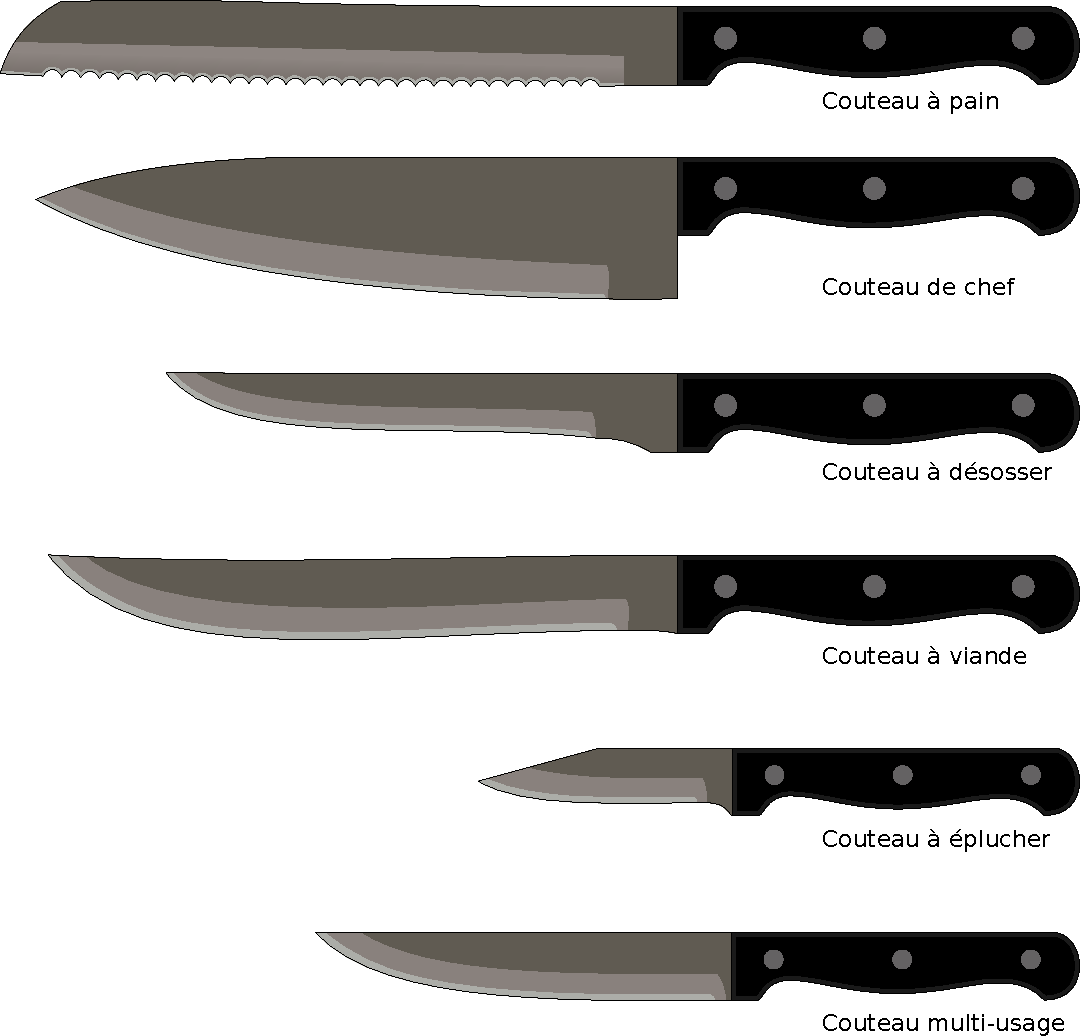
\includegraphics[width=0.6\linewidth]{figures/couteaux.pdf}
\caption{Nom et forme de quelques couteaux de cuisine. À noter que le couteau de chef est un couteau multi-usage aussi.}
\end{figure}

\begin{remarque}
Pour une utilisation optimale, il convient d'aiguiser le couteau avant chaque utilisation à l'aide d'un fusil. Pas besoin d'y passer des heures, quelques mouvements suffisent.

Il faut poser le couteau (près de la garde) sur le fusil, avec une inclinaison d'environ 30\degre, le coté tranchant vers l'avant. Poussez ainsi la lame pour que le fusil rencontre la totalité du fil du couteau. Le mouvement doit être régulier afin de ne pas changer l'angle. Faites ensuite de même en passant sur le dessous du fusil pour l'autre coté du couteau.

Il est important de faire un mouvement pour chaque tranchant du couteau à chaque fois afin que l'affûtage soit homogène.
\end{remarque}

% Pour ma pierre à aiguiser 1000 3000, le coté beige est le coté à 3000, et le coté rouge le coté à 1000. En gros, le coté gros grain est le coté le plus épais.

\section{Herbes aromatiques}
\begin{itemize}
\item Aneth : Son goût anisé est très utilisé pour les recettes à base de poissons et d’œufs. On l’utilise en petite quantité pour agrémenter le plat et on ne soumet pas l’aneth à une cuisson trop forte, pour ne pas en perdre les qualités gustatives.

\item Basilic : Riche en arômes s’accommode parfaitement avec les plats ensoleillés. Avec des légumes, des pâtes ou en salade, le basilic relève vos recettes d’un parfum à la fois doux et intense. On retiendra qu’il est l’élément principal de la fameuse sauce pistou.

\item Ciboulette : les feuilles de ciboulette sont souvent utilisées ciselées dans les sauces et les salades pour les agrémenter d’un goût proche de l’oignon doux. On l’appréciera notamment dans une sauce à la crème fraîche (légère de préférence !) et au poivre pour accompagner une pomme de terre au four.

\item Cumin : Sa saveur chaude et piquante accompagne les fromages, le pain, les carottes et l’agneau.

\item Estragon : les feuilles d’estragon, qu’elles soient utilisées fraîches, séchées ou en poudre s’accommodent particulièrement avec les viandes blanches, le poisson et les œufs.

\item Laurier : originaire d’Europe, la feuille de laurier entre dans la composition des potages, marinades, et civets. Elle accompagne également la composition des bouquets garnis.

\item Marjolaine : autrement nommée \og grand origan\fg, cette plante condimentaire relativement méconnue peut être incorporée à vos ragoûts ou accompagner vos tomates. Son goût étant assez prononcé, il est conseillé d’éviter de la cuire trop longtemps ou de la mélanger à d’autres herbes.

\item Menthe : herbe aromatique phare des cuisines méditerranéennes, la menthe accompagne de nombreuses préparations traditionnelles, avec sa saveur douce et fraîche. Dans le thé ou le taboulé, avec des nems ou dans des desserts, la menthe apporte cette petite touche de vitalité à vos plats.

\item Origan : indispensable sur la pizza napolitaine, très apprécié dans la sauce tomate, l’origan est reconnu pour son goût prononcé et ses vertus médicinales. Souvent confondu avec la marjolaine, dont le goût est plus délicat, les deux plantes ont cependant les mêmes usages.

\item Oseille : avec sa saveur piquante et acidulée, l’oseille qui se cuisine comme les épinards, relève les œufs et les poissons.

\item Persil : riches en vitamines A et C, les feuilles de persil sont utilisées dans les préparations de légumes, avec de la viande ou du poisson. Qu’elles soient plates ou frisées, leur odeur et leur goût sont prononcés.

\item Romarin : son nom signifie en latin rosée de mer, et il pousse à l’état sauvage sur le pourtour méditerranéen. Son odeur camphrée accompagne viandes rôties, pommes de terre ainsi que le vinaigre.

\item Thym : poussant en milieu aride et rocailleux, le thym possède une force olfactive méditerranéenne de caractère. Sa fraîcheur et sa profondeur parfument bouquets garnis, marinades, potages et grillades.
\end{itemize}



\section{Temps de cuisson au four/grill}\index{temps de cuisson}
\begin{table}[htb]
\centering
\begin{tabular}{|c|c|}\hline
Préparation & Temps de cuisson\\\hline\hline
\multicolumn{2}{|c|}{\bsc{Viandes}}\\\hline
B\oe uf & $15\unit{min}/500\unit{g}$\\\hline
Mouton (épaule, gigot) & $15$ à $20\unit{min}/500\unit{g}$\\\hline
Porc,veau & $30$ à $35\unit{min}/500\unit{g}$\\\hline\hline
\multicolumn{2}{|c|}{\bsc{Volailles}}\\\hline
Poulet & $25$ à $30\unit{min}/500\unit{g}$\\\hline
Caille & $20$ à $25\unit{min}$\\\hline
\end{tabular}
\caption{Cuisson Grill/rotissoire (Garder la porte entrouverte)}
\end{table}

\begin{table}[htb]
\centering
\begin{tabular}{|c|c|c|c|}\hline
Préparation & Thermostat \degres C & Temps de Cuisson & Remarques\\\hline\hline
\multicolumn{4}{|c|}{\bsc{Entrées}}\\\hline
Soufflé au fromage & 200 & 35\unit{min} & Plat en terre ou verre\\\hline
Quiche lorraine & 240 & 45\unit{min} & Moule à tarte\\\hline
Tomates farcies & 240 & 50\unit{min} & Plat en terre ou verre\\\hline
Gratin Dauphinois & 240 & 50\unit{min} & Plat en terre ou verre\\\hline
Pizza & 240 & 35\unit{min} & Plaque à pâtisserie\\\hline
\OE ufs cocotte & 270 & 8 à 10\unit{min} & Ramequin et bain-marie\\\hline
Allumettes fromage & 260 & 10\unit{min} & Plaque à pâtisserie\\\hline
Croque-Monsieur & 220 & 20\unit{min} & Grille\\\hline\hline
\multicolumn{4}{|c|}{\bsc{Viandes}}\\\hline
B\oe uf & 270 & 15\unit{min}/500\unit{g} & Plat en terre\\\hline
Mouton (épaule, gigot) & 270 & 15\unit{min}/500\unit{g} & Plat en terre\\\hline
Porc,veau & 250 & 30 à 35\unit{min}/500\unit{g} & Plat en terre\\\hline
Agneau & 210 & 12\unit{min}/500\unit{g} & Plat en terre\\\hline\hline
\multicolumn{4}{|c|}{\bsc{Poissons}}\\\hline
Truite (1\unit{kg}) & 240 & 35\unit{min} & Plat en terre ou verre\\\hline
Maquereaux & 240 & 30\unit{min} & Plat en terre ou verre\\\hline\hline
\multicolumn{4}{|c|}{\bsc{Volailles}}\\\hline
Poulet & 260 & 25 à 30\unit{min}/500\unit{g} & Plat en terre\\\hline
Lapin & 240 & 25 à 30\unit{min}/500\unit{g} & Plat en terre\\\hline\hline
\multicolumn{4}{|c|}{\bsc{Pâtisseries}}\\\hline
Biscuit de Savoie & 170 & 35\unit{min} & Moule à manqué\\\hline
\multirow{3}*{Cake} & 220 & 15\unit{min} & \multirow{3}*{Moule à cake}\\
&\multicolumn{2}{c|}{puis} &\\
&180 & 55\unit{min} &\\\hline
Clafoutis & 240 & 50\unit{min} & Moule à manqué\\\hline
Quatre-quart & 160 & 60\unit{min} & Moule à cake\\\hline
Sablés & 190 & 15\unit{min} & Plaque à pâtisserie\\\hline
Pâte brisée garnie & 230 & 35\unit{min} & Moule\\\hline
Pommes au four & 230 & 25 à 30\unit{min} & Plat en terre ou verre\\\hline
Meringues & 110 & 120\unit{min} & Plaque à pâtisserie\\\hline
\end{tabular}
\caption{Cuisson Four}
\end{table}


\end{document}